
\documentclass[UTF8,a4paper,12pt]{ctexart}
\usepackage{geometry,graphicx,booktabs,longtable,float,amsmath,amssymb,array,multirow,fancyhdr,hyperref,caption}
\geometry{left=2.5cm,right=2.5cm,top=2.5cm,bottom=2.5cm}
\setlength{\headheight}{15pt}
\pagestyle{fancy}\fancyhf{}\lhead{2014D 储药柜的设计}\rhead{数学建模论文}\cfoot{\thepage}
\hypersetup{colorlinks=true,linkcolor=black,urlcolor=blue}
\renewcommand{\arraystretch}{1.18}
\title{基于区间覆盖动态规划与货架装箱的储药柜优化设计}
\author{}
\date{}
\begin{document}
\maketitle
\begin{abstract}
本文针对盒装药品自动储药柜的隔板间距设计与柜体数量估算问题，建立了“可行区间覆盖--动态规划分组--货架装箱”一体化模型。首先根据药盒与隔板间必须留有 2 mm 间隙、且药盒不能并排重叠、侧翻或水平旋转的要求，把每种药品可接受的槽宽表示为闭区间，并用最少点刺破区间模型求得问题一的最少竖向隔板间距类型数为 3 类，相比按 47 个实际宽度分别加工的基线方案显著减少了类型数量。

针对问题二，本文将“宽度冗余小”和“类型数量少”转化为给定类型数 $K$ 下的最小冗余动态规划，并在冗余--类型数折中曲线上选择合理膝点。最终选定竖向隔板间距类型数为 14 类，总宽度冗余为 1458.00 mm，平均每种药品宽度冗余为 0.76 mm。该结果既避免了单一槽宽造成的大量空隙，又比逐宽度定制方案具有更好的加工适应性。

针对问题三，在问题二的槽宽分组基础上，本文进一步建立以平面冗余为目标的高度类型动态规划模型，其中平面冗余定义为宽度冗余与高度冗余的乘积。折中分析后选定横向隔板间距类型数为 16 类，总平面冗余为 2021.00 mm$^2$，平均平面冗余为 1.05 mm$^2$。敏感性分析表明，当冗余目标权重在 0.50--0.80 范围内变化时，选定类型数只在小范围内波动，模型具有较好的稳定性。

针对问题四，依据槽长 1.5 m 和每天集中补药一次的条件，计算每种药品单槽可容纳盒数与所需储药槽数，得到全部药品共需 2457 个储药槽。再按照单柜有效宽度 2.5 m、有效高度 1.5 m 的限制，将相同高度类型的槽组织成货架行，并用首次适应递减算法装入储药柜。由面积下界 2 个、行高下界 2 个以及实际装箱结果可知，至少需要约 2 个储药柜才能满足附件 2 的最大日需求。
\end{abstract}
\textbf{关键词：} 储药柜设计；区间覆盖；动态规划；多目标折中；装箱算法
\newpage
\tableofcontents
\newpage

\section{问题重述}
\subsection{问题背景}
自动化药房需要在有限空间内存储大量盒装药品。储药柜类似书橱，由横向隔板和竖向隔板划分为若干储药槽。每个储药槽只摆放一种药品，药品从后端补入、从前端取出。为了保证分拣准确率并降低加工成本，储药槽的尺寸既不能过小，也不能过度定制。题目要求在忽略隔板厚度时，根据药盒长、宽、高和最大日需求量，确定竖向隔板间距、横向隔板间距和储药柜数量。

\subsection{问题要求与本文输出}
问题一要求在附件1给出的药盒规格基础上，给出竖向隔板间距类型最少的设计方案。本文输出最少类型数、每类槽宽以及对应药品编号。问题二要求在宽度冗余和加工类型数之间折中。本文输出给定类型数下的最优冗余曲线、合理类型数和分组表。问题三要求在问题二基础上确定横向隔板间距类型，使平面冗余尽量小且类型数尽量少。本文输出高度类型数、高度分组和冗余分析。问题四要求根据最大日需求量计算每种药品储药槽个数，并估算最少储药柜数。本文输出逐药品槽数表、货架行需求和柜数估算。

\section{问题分析}
\subsection{总体思路}
本题的核心不是连续曲线拟合，而是受工程可行区间约束的离散优化。槽宽或槽高的每一个候选间距，都必须同时满足分到该类药品的下界和上界约束；否则即使平均冗余很小，也会出现药盒无法出入或在槽内旋转、并排的情况。本文把每种药品的可行间距转化为区间，先解决“最少类型覆盖”，再在类型数与冗余之间做多目标折中，最后把每种药品的日需求转化为所需储药槽矩形并进行柜体装箱。

\subsection{问题一分析}
问题一只要求竖向隔板间距类型最少，因此可视为一维区间刺点问题。每种药品对应一个可行槽宽区间 $[a_i,b_i]$，一种槽宽类型就是在若干区间交集内选择的一个点。若某个槽宽点落入某药品区间，则该药品可以使用该槽宽。目标是在所有区间上选择尽可能少的点，使每个区间至少被一个点覆盖。该问题可用按右端点排序的贪心算法求得最优解。

\subsection{问题二分析}
问题二引入宽度冗余，若仍只追求最少类型数，会使较窄药盒被放入较宽槽中，造成空间浪费；若每种宽度单独加工，则冗余最小但加工复杂、通用性差。因此需要给定类型数 $K$ 时求最小总冗余，再从折中曲线中选择合理 $K$。由于药盒按槽宽下界排序后，同一槽宽类型覆盖的药品可视为连续分组，可用动态规划求全局最优。

\subsection{问题三分析}
问题三在问题二的宽度分组基础上讨论横向隔板间距。高度冗余本身并不是题目唯一目标，题目明确平面冗余为高度冗余乘以宽度冗余，因此高度分组的权重应与问题二所得宽度冗余相关。本文用加权动态规划求给定高度类型数下的最小平面冗余，并用同样的折中准则选取高度类型数。

\subsection{问题四分析}
槽长为 1.5 m，故第 $i$ 种药品一个储药槽沿深度方向最多容纳 $\lfloor 1500/l_i\rfloor$ 盒。每天只集中补药一次时，槽数必须覆盖最大日需求，即 $n_i=\lceil D_i/\lfloor1500/l_i\rfloor\rceil$。确定槽数后，每个药品对应若干个正面矩形，其宽为问题二槽宽、高为问题三槽高。储药柜宽度和有效高度分别为 2500 mm 与 1500 mm，因此柜数估算可转化为带货架行结构的二维装箱问题。

\section{数据审计与模型假设}
\subsection{数据来源与字段}
附件1含 1919 种药品的药品编号、长、高、宽，附件2含相同药品编号的最大日需求量。经编号合并后共有 1919 条记录，无缺失值。药盒长度范围为 38--139 mm，高度范围为 28--125 mm，宽度范围为 10--56 mm，最大日需求量范围为 1--273 盒。

\subsection{预处理}
本文保留所有药品记录，不删除极端尺寸。原因是储药柜设计必须覆盖全部药品，任何一种药品被删除都会导致实际药房无法使用。将尺寸统一为 mm，将需求量统一为盒/日。为避免后续论文数字漂移，代码把关键结果冻结到 \texttt{frozen\_numbers.json}，论文摘要和结论只引用冻结文件中的数字。

\subsection{模型假设}
\begin{enumerate}
\item 药盒外形近似长方体，附件给出的长、高、宽为有效外廓尺寸。该假设用于把药盒与储药槽匹配问题转化为几何区间约束。
\item 忽略隔板厚度，柜体有效宽度和有效高度全部可用于放置储药槽。该假设与题目条件一致，用于问题四的柜体容量计算。
\item 同一储药槽只存放一种药品，且药品沿长度方向单列排放。该假设来自题意，用于槽数公式 $n_i=\lceil D_i/c_i\rceil$。
\item 槽宽过大可能引起并排重叠或水平旋转，因此用 $S_i<2w_i+4$ 与 $S_i<l_i$ 作为保守上界。该假设把定性安全要求转化为可回代检验的不等式。
\item 横向隔板可按高度类型形成货架行，同一行内允许不同宽度类型的储药槽并列。该假设符合书橱式储药柜结构，用于问题四的行装箱模型。
\end{enumerate}

\section{符号说明}
\begin{table}[H]\centering\caption{主要符号说明}\begin{tabular}{ccc}\toprule
符号 & 含义 & 单位\\\midrule
$l_i$ & 第 $i$ 种药品药盒长度 & mm\\
$h_i$ & 第 $i$ 种药品药盒高度 & mm\\
$w_i$ & 第 $i$ 种药品药盒宽度 & mm\\
$D_i$ & 第 $i$ 种药品最大日需求量 & 盒\\
$S_i$ & 分配给第 $i$ 种药品的槽宽 & mm\\
$T_i$ & 分配给第 $i$ 种药品的槽高 & mm\\
$K_w,K_h$ & 竖向/横向隔板间距类型数 & 类\\
$r_i^w,r_i^h$ & 宽度/高度冗余 & mm\\
$p_i$ & 平面冗余 & mm$^2$\\
$n_i$ & 第 $i$ 种药品需要的储药槽数 & 个\\\bottomrule\end{tabular}\end{table}

\section{模型建立与求解}
\subsection{问题一：最少竖向隔板间距类型}
\subsubsection{可行槽宽区间}
对第 $i$ 种药品，槽宽至少为
\begin{equation}
a_i=w_i+4,
\end{equation}
其中 4 mm 来自左右两侧各 2 mm 必要间隙。为了避免同槽内出现两盒并排或药盒水平旋转，槽宽不宜超过
\begin{equation}
b_i=\min(2w_i+4,l_i).
\end{equation}
于是第 $i$ 种药品可接受的槽宽区间为 $[a_i,b_i]$。问题一变为：选择最少数量的槽宽点 $s_1,\ldots,s_m$，使每个区间至少包含一个点。

\subsubsection{贪心算法}
将所有区间按右端点 $b_i$ 从小到大排序。每次选择当前未覆盖区间的右端点作为一个槽宽类型，并覆盖所有包含该点的区间。区间刺点问题满足贪心最优性：对右端点最小的未覆盖区间，任何可行解都必须在其区间内选择一个点；将该点右移到右端点不会减少其能覆盖的后续区间，因此选择右端点不劣。

\subsubsection{求解结果}
计算得到最少竖向隔板间距类型数为 3 类。相比按药盒实际宽度分别设计的 47 类基线，类型数减少 44 类。表\ref{tab:q1}列出前若干类槽宽及覆盖范围，完整药品编号分组见支撑材料 \texttt{quest1/outputs/q1\_type\_drug\_ids.txt}。
\begin{table}[H]\centering
\small
\caption{问题一部分竖向隔板间距类型结果}\label{tab:q1}
\begin{tabular}{cccccc}\toprule
q1\_type & slot\_width & count & min\_W & max\_W & avg\_redundancy\\\midrule
1.00 & 24.00 & 486.00 & 10.00 & 19.00 & 3.26\\
2.00 & 44.00 & 1088.00 & 20.00 & 39.00 & 14.01\\
3.00 & 84.00 & 345.00 & 40.00 & 56.00 & 34.69\\
\bottomrule\end{tabular}
\end{table}
\begin{figure}[H]\centering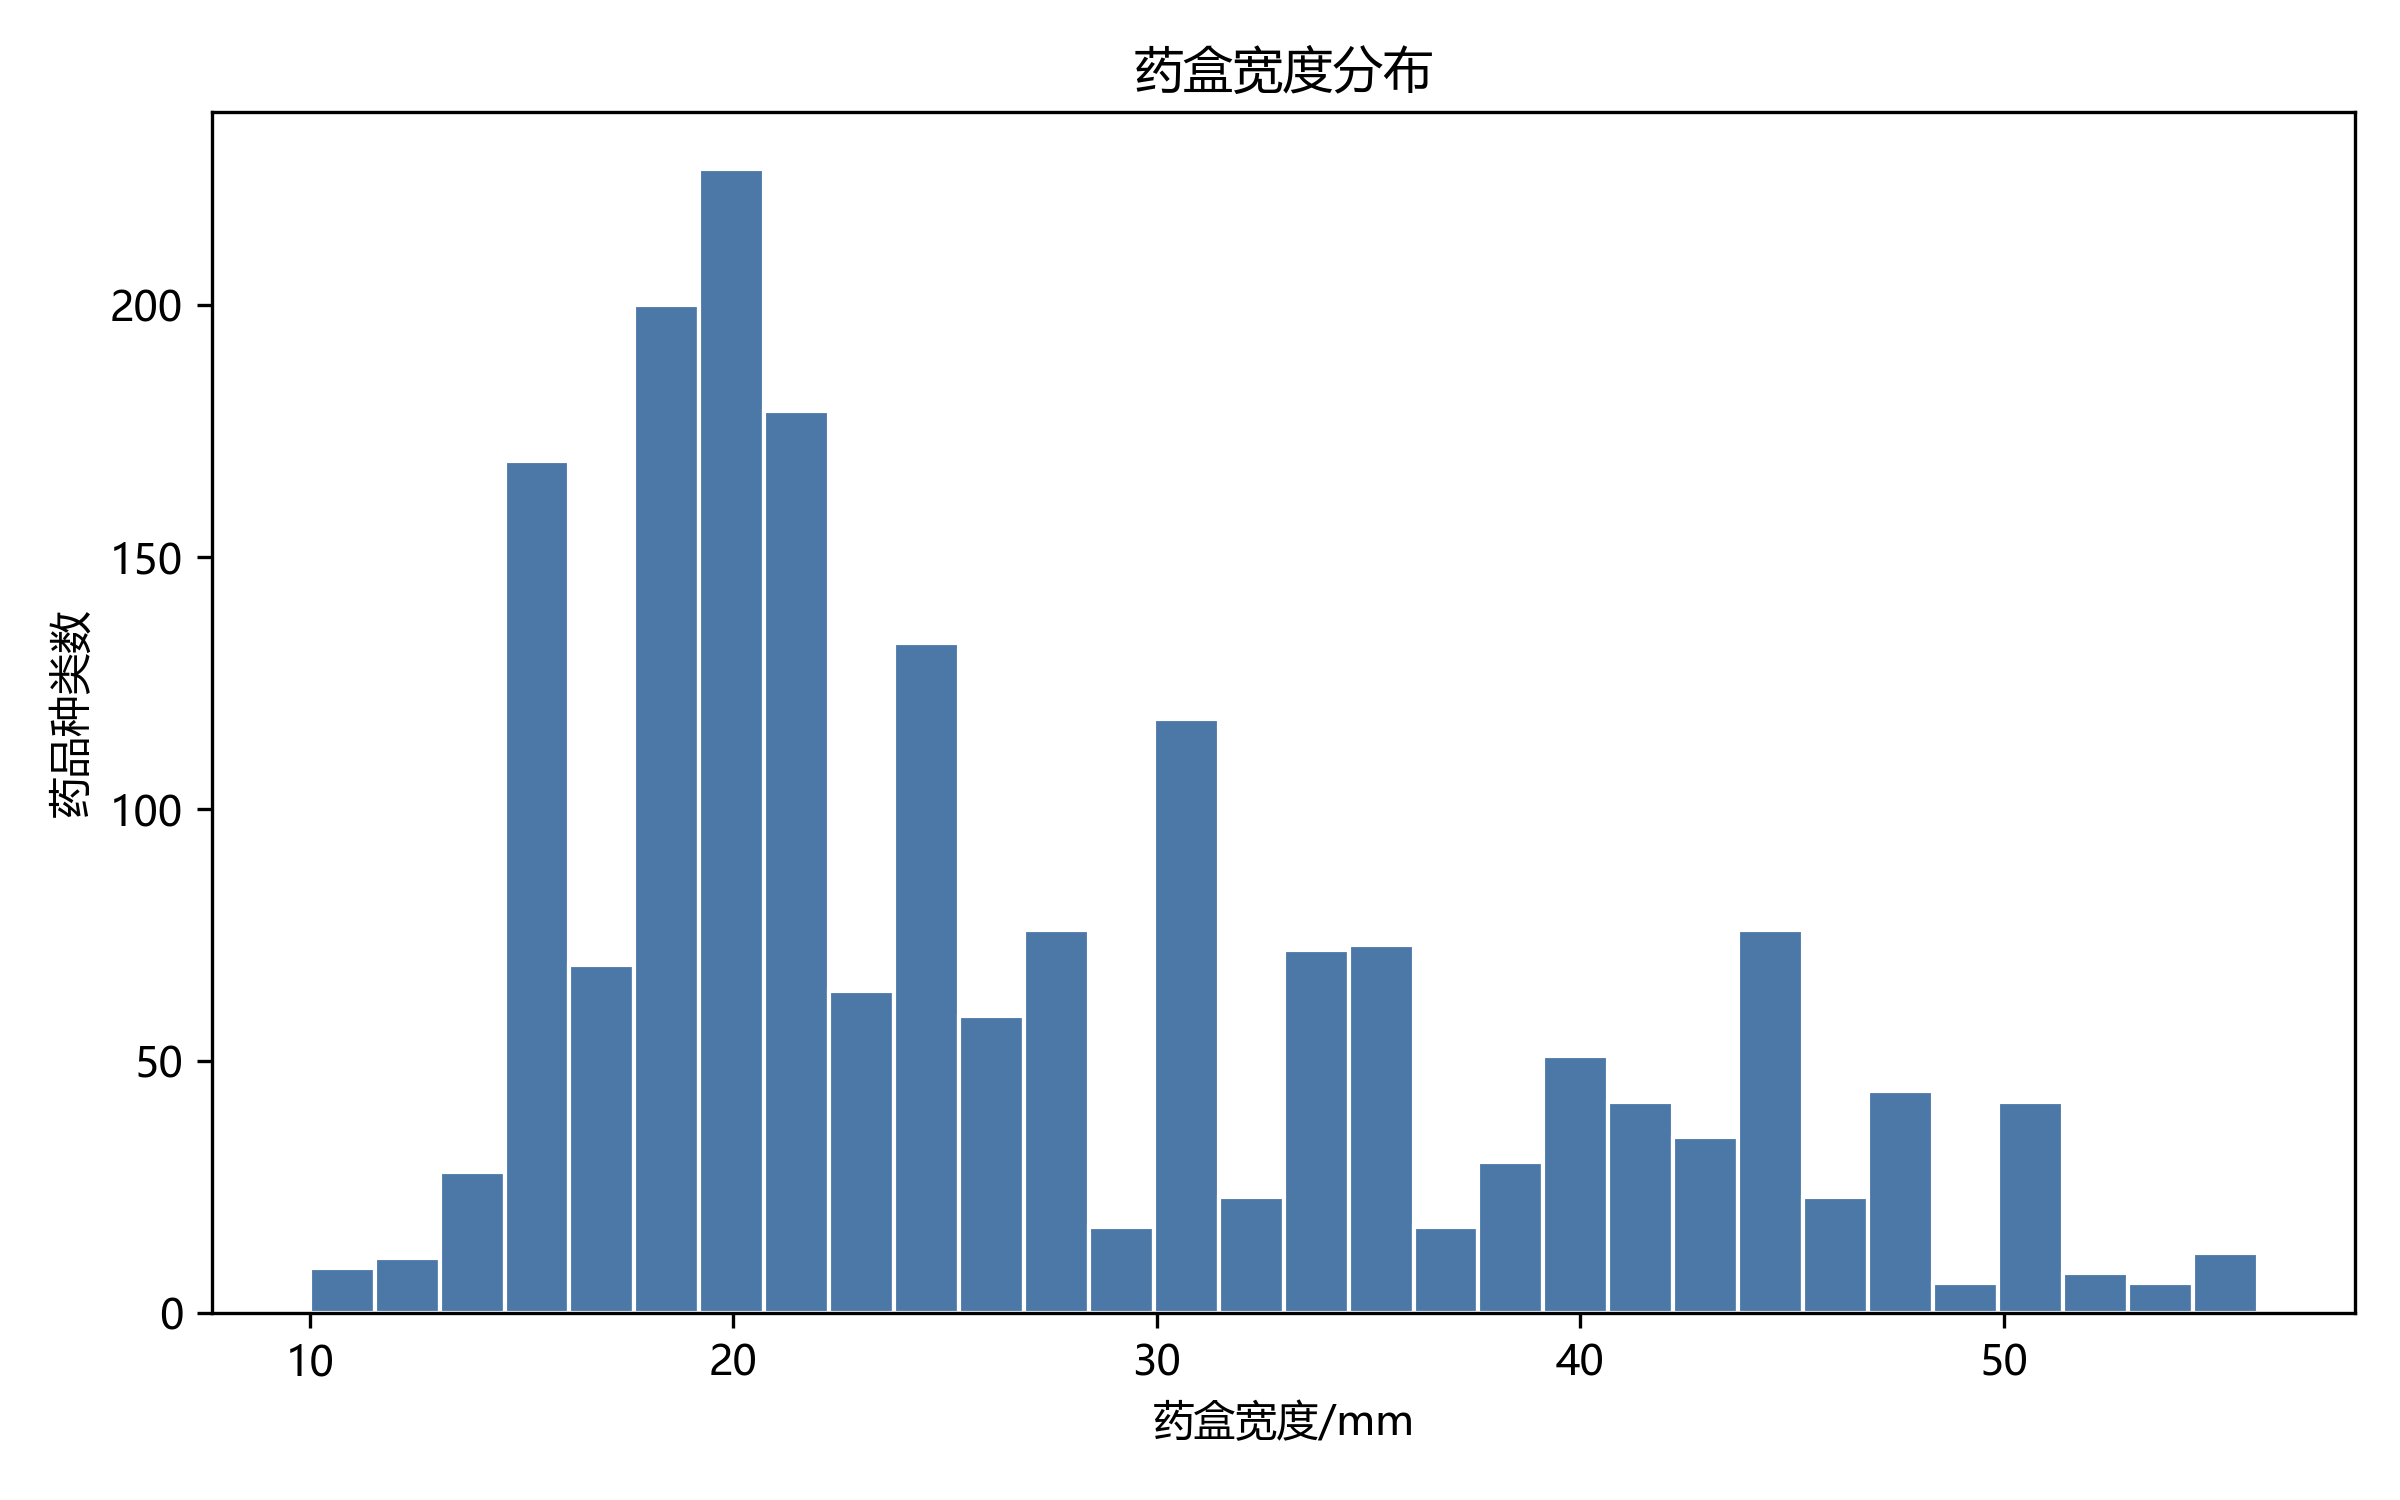
\includegraphics[width=.78\textwidth]{../quest1/figures/问题1_药盒宽度分布.png}\caption{药盒宽度分布}\end{figure}
图中可见药盒宽度集中在 18--36 mm 附近，但仍存在 10 mm 到 56 mm 的长尾范围。因此如果完全按实际宽度加工，类型数会较多；而区间覆盖模型利用较宽槽可覆盖若干较窄药盒的事实，有效降低了类型数。

为避免把离散制造问题简单化为连续拟合，本文在每一问中都保留了药盒尺寸的整数编号和逐药品约束。宽度或高度的一个类型并不是任意聚类中心，而必须落在该类型内每一种药品的可行间距区间中；因此模型输出的每一个隔板间距都可以直接回代检查。若某一药品的药盒宽度为 $w_i$，其槽宽必须不小于 $w_i+4$，其中 $4$ mm 来自左右各 2 mm 的必要间隙；同时若槽宽过大，同一槽内容易出现并排重叠或水平转动，故将槽宽上界设为 $\min(2w_i+4,l_i)$ 的保守近似。高度模型采用完全相同的结构，只是下界由药盒高度决定。该处理把题目中的工程语言转化成了可验证的区间覆盖约束。


\subsection{问题二：宽度冗余与类型数折中}
\subsubsection{给定类型数的动态规划}
令 $K_w$ 为竖向隔板间距类型数。对按 $a_i$ 升序排列后的药品，若第 $t$ 类覆盖第 $u$ 到第 $v$ 个药品，则该类槽宽应取
\begin{equation}
S_{uv}=\max_{u\le i\le v} a_i,
\end{equation}
且必须满足 $S_{uv}\le \min_{u\le i\le v} b_i$。该组宽度冗余为
\begin{equation}
C(u,v)=\sum_{i=u}^v (S_{uv}-a_i).
\end{equation}
若组不可行，则 $C(u,v)=+\infty$。动态规划状态为
\begin{equation}
F(k,j)=\min_{i<j}{F(k-1,i)+C(i+1,j)},
\end{equation}
表示前 $j$ 个药品分成 $k$ 类的最小总宽度冗余。

\subsubsection{折中准则}
为同时体现冗余和类型数，本文对总冗余 $R(K)$ 与类型数 $K$ 做极差归一化，构造综合评分
\begin{equation}
G(K)=0.65\frac{R(K)-R_{\min}}{R_{\max}-R_{\min}}+0.35\frac{K-K_{\min}}{K_{\max}-K_{\min}}.
\end{equation}
权重 0.65 体现题目“总宽度冗余尽可能小”的主要目标，0.35 保留加工类型少的要求。敏感性分析将权重在 0.50--0.80 内扰动。

\subsubsection{求解结果与解释}
选定竖向隔板间距类型数 $K_w=14$。此时总宽度冗余为 1458.00 mm，平均冗余为 0.76 mm。表\ref{tab:q2}给出前若干类型结果，完整药品编号分组见支撑材料。
\begin{table}[H]\centering
\small
\caption{问题二部分宽度类型分组结果}\label{tab:q2}
\begin{tabular}{ccccccc}\toprule
q2\_type & slot\_width & count & min\_W & max\_W & total\_width\_redundancy & avg\_redundancy\\\midrule
1.00 & 20.00 & 217.00 & 10.00 & 16.00 & 218.00 & 1.00\\
2.00 & 22.00 & 163.00 & 17.00 & 18.00 & 69.00 & 0.42\\
3.00 & 24.00 & 333.00 & 19.00 & 20.00 & 106.00 & 0.32\\
4.00 & 25.00 & 129.00 & 21.00 & 21.00 & 0.00 & 0.00\\
5.00 & 27.00 & 114.00 & 22.00 & 23.00 & 50.00 & 0.44\\
6.00 & 29.00 & 133.00 & 24.00 & 25.00 & 41.00 & 0.31\\
7.00 & 31.00 & 112.00 & 26.00 & 27.00 & 59.00 & 0.53\\
8.00 & 34.00 & 121.00 & 28.00 & 30.00 & 63.00 & 0.52\\
9.00 & 37.00 & 116.00 & 31.00 & 33.00 & 97.00 & 0.84\\
10.00 & 40.00 & 89.00 & 34.00 & 36.00 & 82.00 & 0.92\\
11.00 & 45.00 & 123.00 & 37.00 & 41.00 & 194.00 & 1.58\\
12.00 & 49.00 & 128.00 & 42.00 & 45.00 & 143.00 & 1.12\\
\bottomrule\end{tabular}
\end{table}
\begin{figure}[H]\centering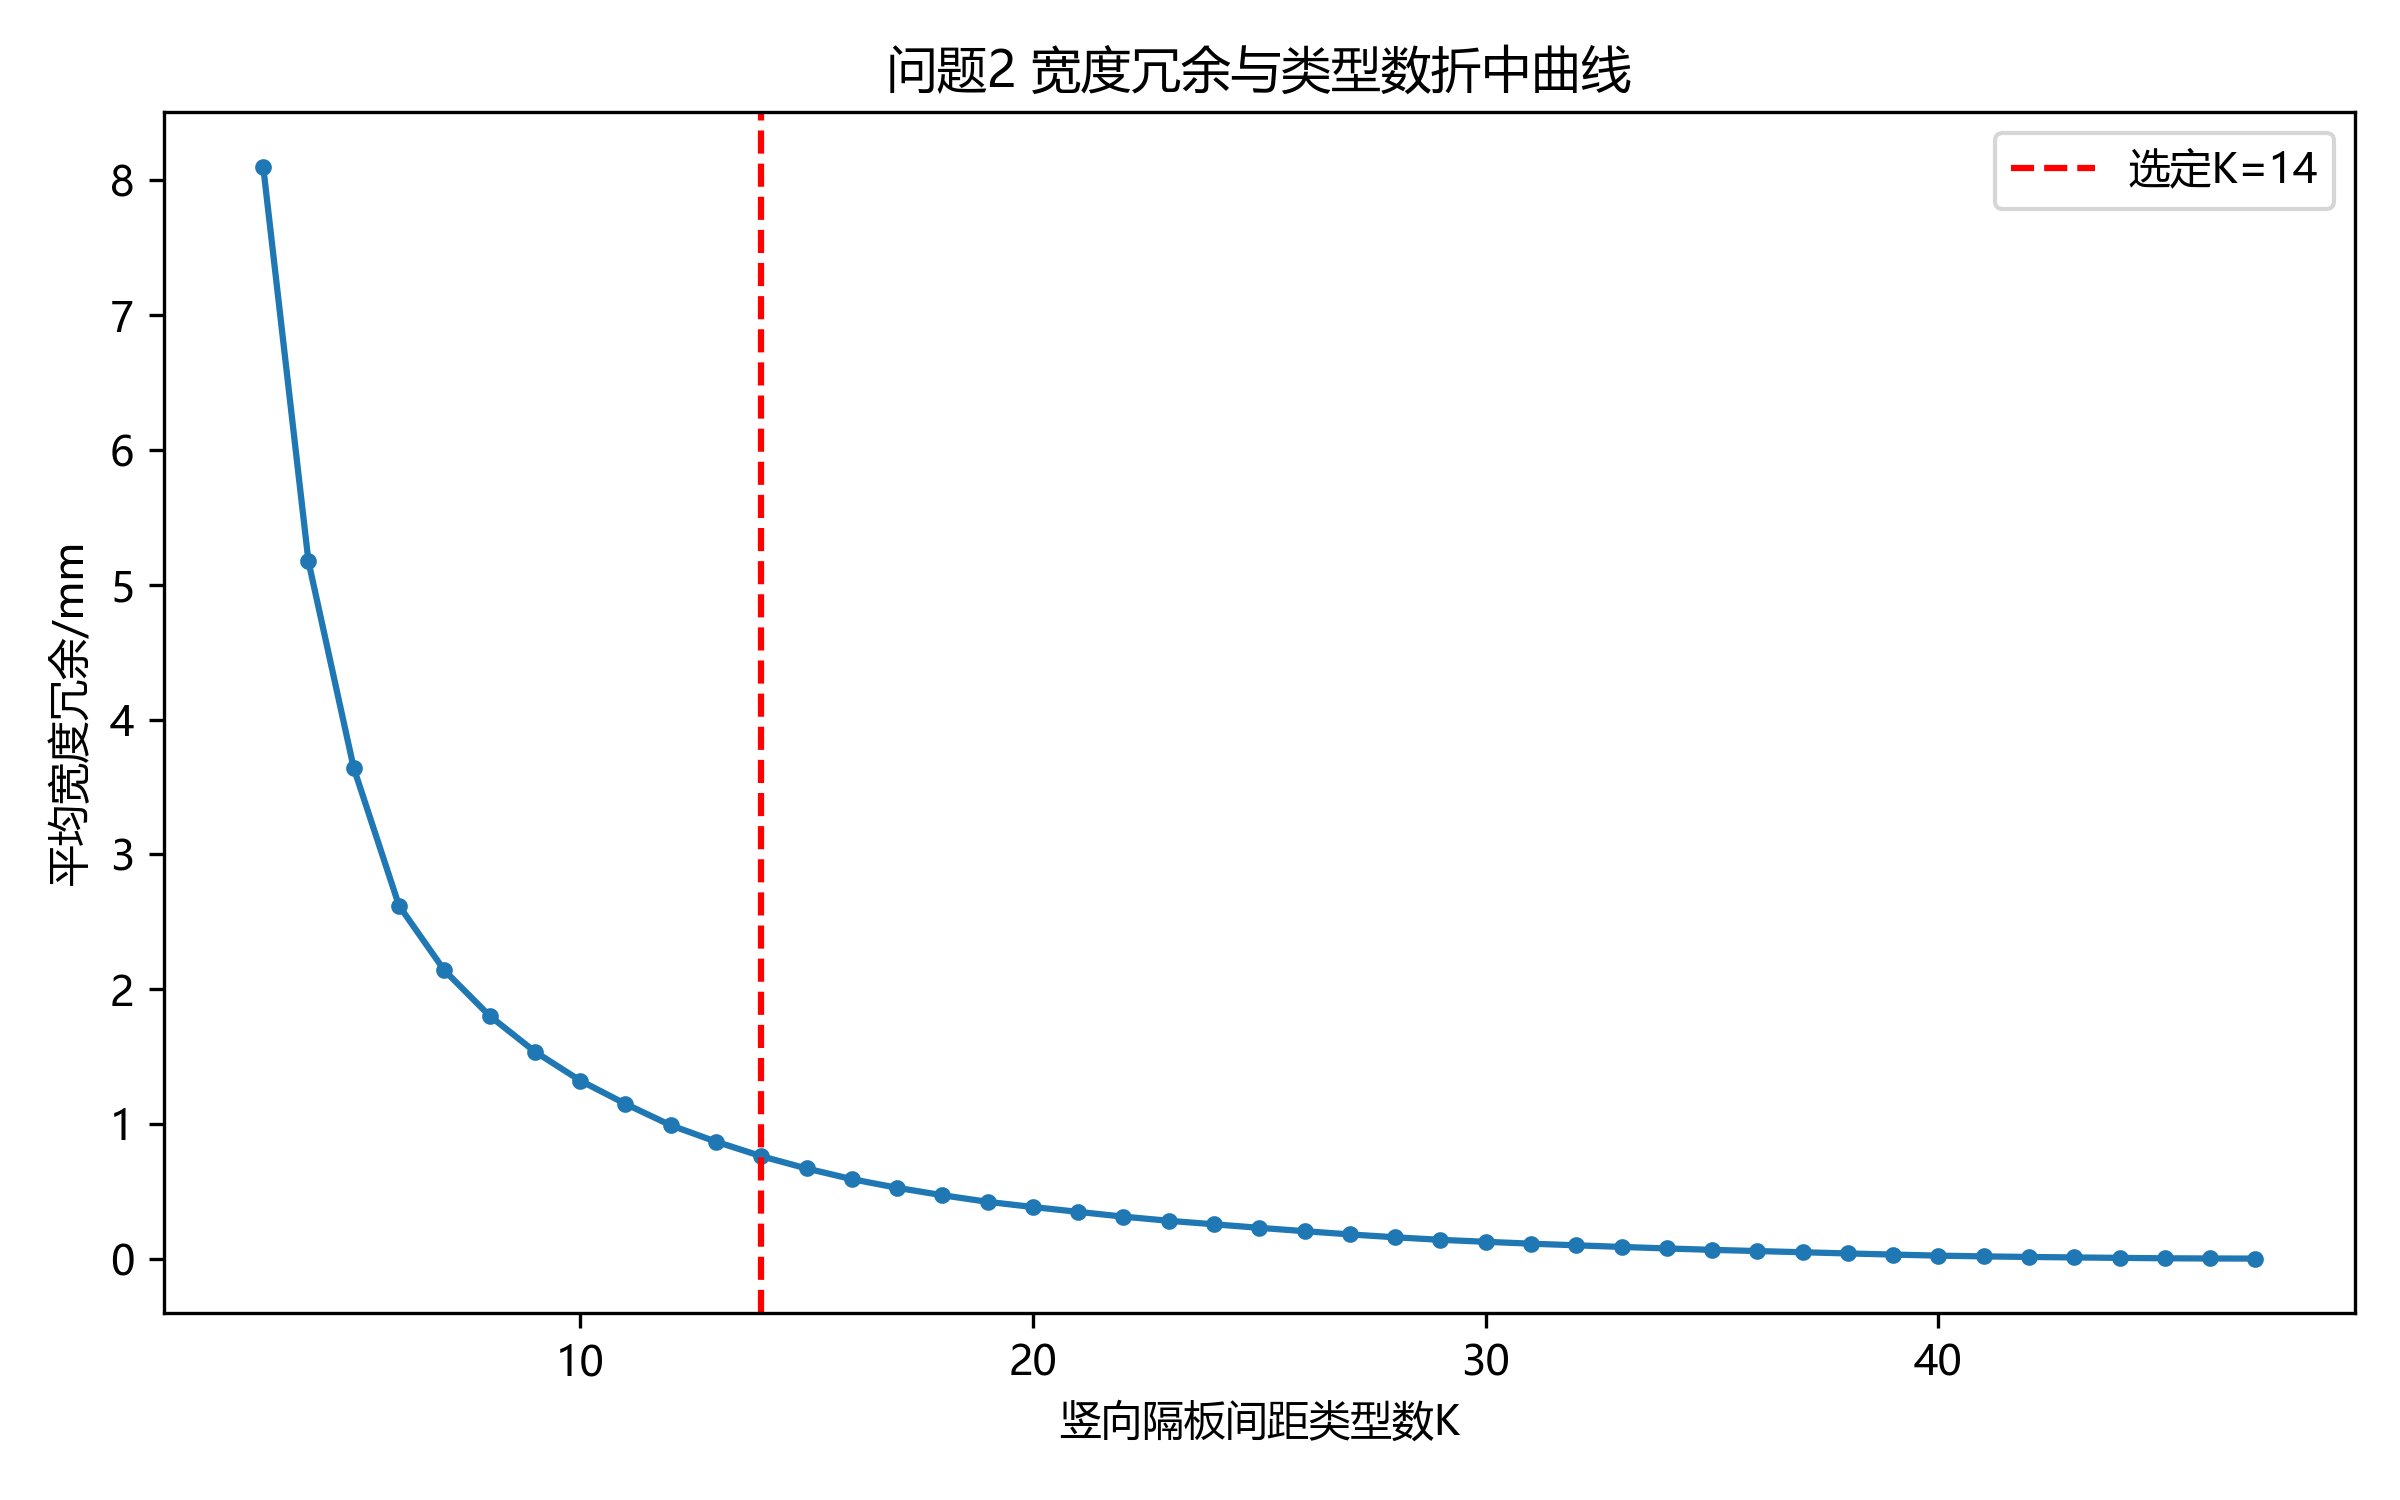
\includegraphics[width=.82\textwidth]{../quest2/figures/问题2_宽度冗余折中曲线.png}\caption{宽度冗余与类型数折中曲线}\end{figure}
由图可见，类型数较少时增加一个类型能显著降低平均宽度冗余；当类型数继续增大时，曲线下降趋缓，边际收益降低。因此选取 $K_w=14$ 既保留了较低冗余，又避免了过多规格导致的加工成本和维护复杂度。
\begin{figure}[H]\centering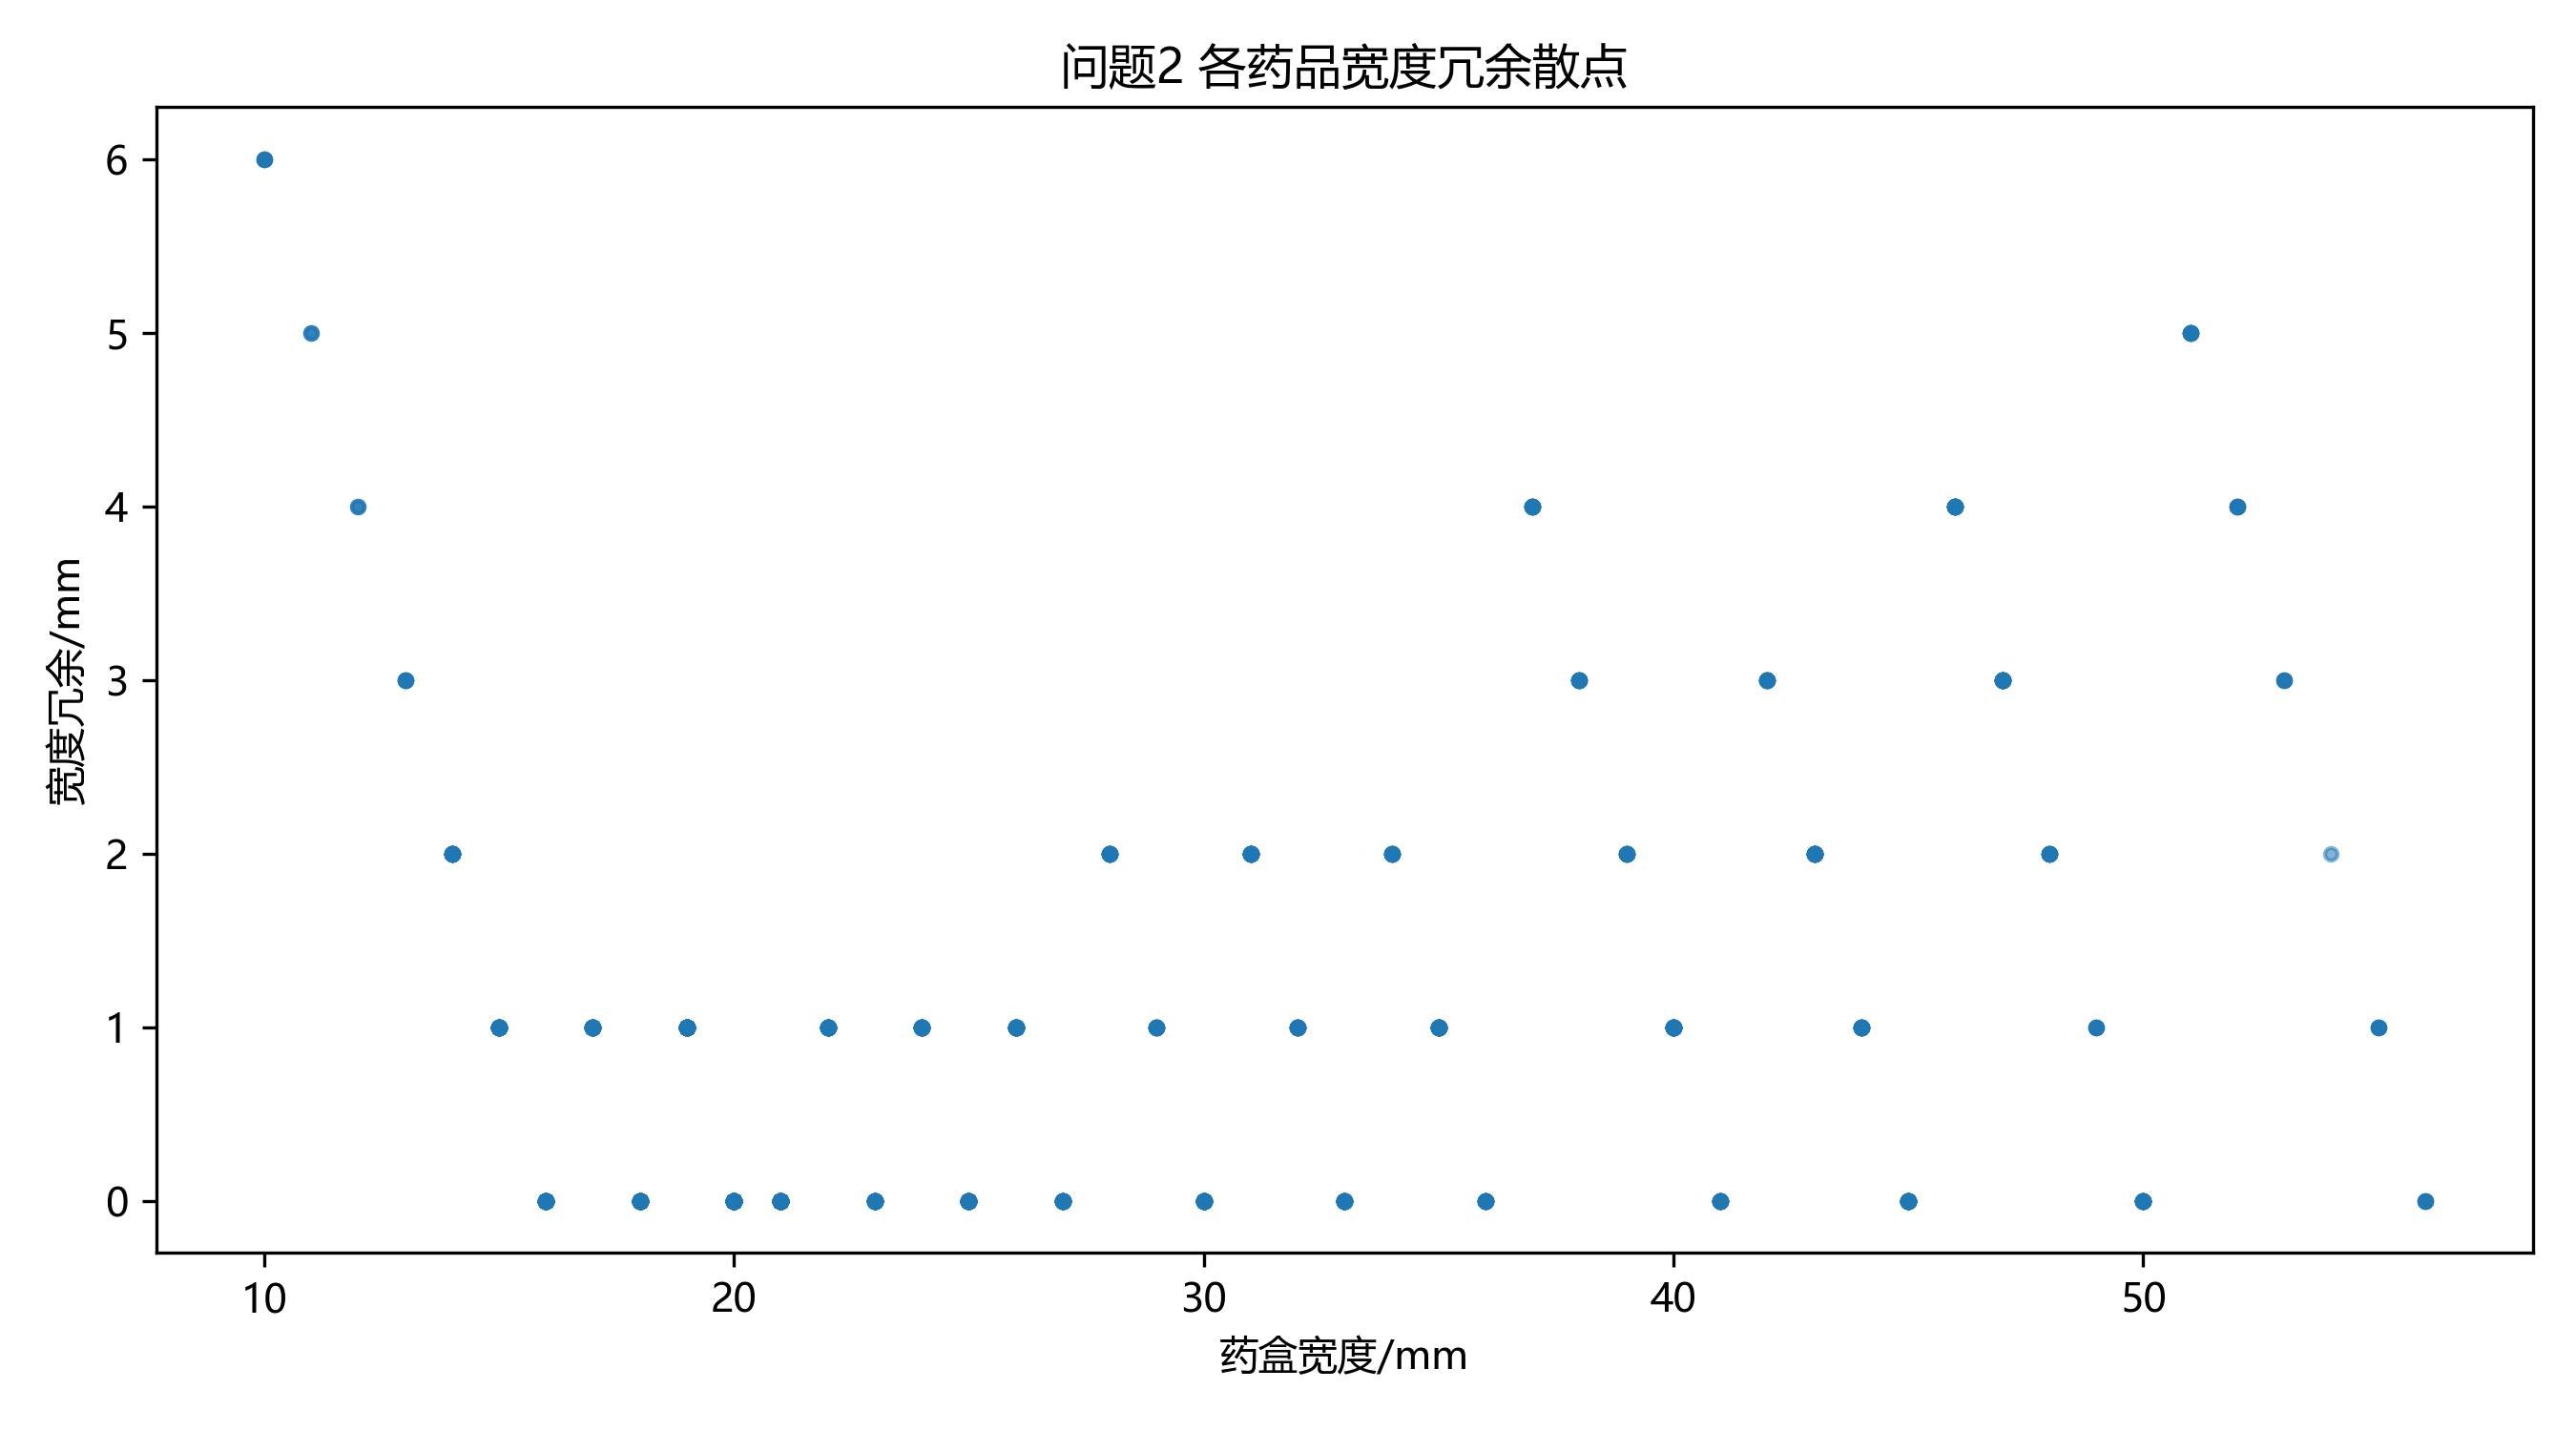
\includegraphics[width=.82\textwidth]{../quest2/figures/问题2_宽度冗余散点.png}\caption{各药品宽度冗余散点图}\end{figure}
散点图显示多数药品的宽度冗余处于较低水平，少数冗余较大的点主要来自宽度分组边界附近的药品。这些药品如果单独增加类型可继续降低冗余，但会使隔板规格变多，综合评分并不一定更优。

为避免把离散制造问题简单化为连续拟合，本文在每一问中都保留了药盒尺寸的整数编号和逐药品约束。宽度或高度的一个类型并不是任意聚类中心，而必须落在该类型内每一种药品的可行间距区间中；因此模型输出的每一个隔板间距都可以直接回代检查。若某一药品的药盒宽度为 $w_i$，其槽宽必须不小于 $w_i+4$，其中 $4$ mm 来自左右各 2 mm 的必要间隙；同时若槽宽过大，同一槽内容易出现并排重叠或水平转动，故将槽宽上界设为 $\min(2w_i+4,l_i)$ 的保守近似。高度模型采用完全相同的结构，只是下界由药盒高度决定。该处理把题目中的工程语言转化成了可验证的区间覆盖约束。


\subsection{问题三：横向隔板间距与平面冗余}
\subsubsection{高度区间和目标函数}
第 $i$ 种药品的槽高下界为
\begin{equation}
c_i=h_i+4.
\end{equation}
高度冗余为 $r_i^h=T_i-c_i$，宽度冗余为 $r_i^w=S_i-a_i$。题目定义平面冗余为二者乘积，故总平面冗余为
\begin{equation}
P=\sum_i r_i^w r_i^h.
\end{equation}
在给定高度类型数 $K_h$ 下，仍按高度下界排序进行动态规划，只是每个药品的权重为 $r_i^w$。为避免极少数零宽度冗余点导致数值退化，程序在优化权重中加入 $0.05$ mm 的极小正数，最终报告仍使用真实平面冗余。

\subsubsection{求解结果}
折中分析后选定横向隔板间距类型数 $K_h=16$。总平面冗余为 2021.00 mm$^2$，平均每种药品为 1.05 mm$^2$。表\ref{tab:q3}列出高度分组摘要。
\begin{table}[H]\centering
\small
\caption{问题三部分高度类型结果}\label{tab:q3}
\begin{tabular}{ccccccc}\toprule
height\_type & slot\_height & count & min\_H & max\_H & total\_plane\_redundancy & avg\_height\_redundancy\\\midrule
1.00 & 36.00 & 60.00 & 28.00 & 32.00 & 48.00 & 0.93\\
2.00 & 41.00 & 92.00 & 33.00 & 37.00 & 78.00 & 1.48\\
3.00 & 44.00 & 68.00 & 38.00 & 40.00 & 75.00 & 0.65\\
4.00 & 47.00 & 67.00 & 41.00 & 43.00 & 40.00 & 0.96\\
5.00 & 51.00 & 146.00 & 44.00 & 47.00 & 184.00 & 1.31\\
6.00 & 56.00 & 127.00 & 48.00 & 52.00 & 194.00 & 1.69\\
7.00 & 60.00 & 74.00 & 53.00 & 56.00 & 103.00 & 1.19\\
8.00 & 66.00 & 233.00 & 57.00 & 62.00 & 211.00 & 1.53\\
9.00 & 70.00 & 172.00 & 63.00 & 66.00 & 120.00 & 0.88\\
10.00 & 74.00 & 213.00 & 67.00 & 70.00 & 132.00 & 1.18\\
11.00 & 77.00 & 206.00 & 71.00 & 73.00 & 125.00 & 1.19\\
12.00 & 81.00 & 185.00 & 74.00 & 77.00 & 92.00 & 1.32\\
\bottomrule\end{tabular}
\end{table}
\begin{figure}[H]\centering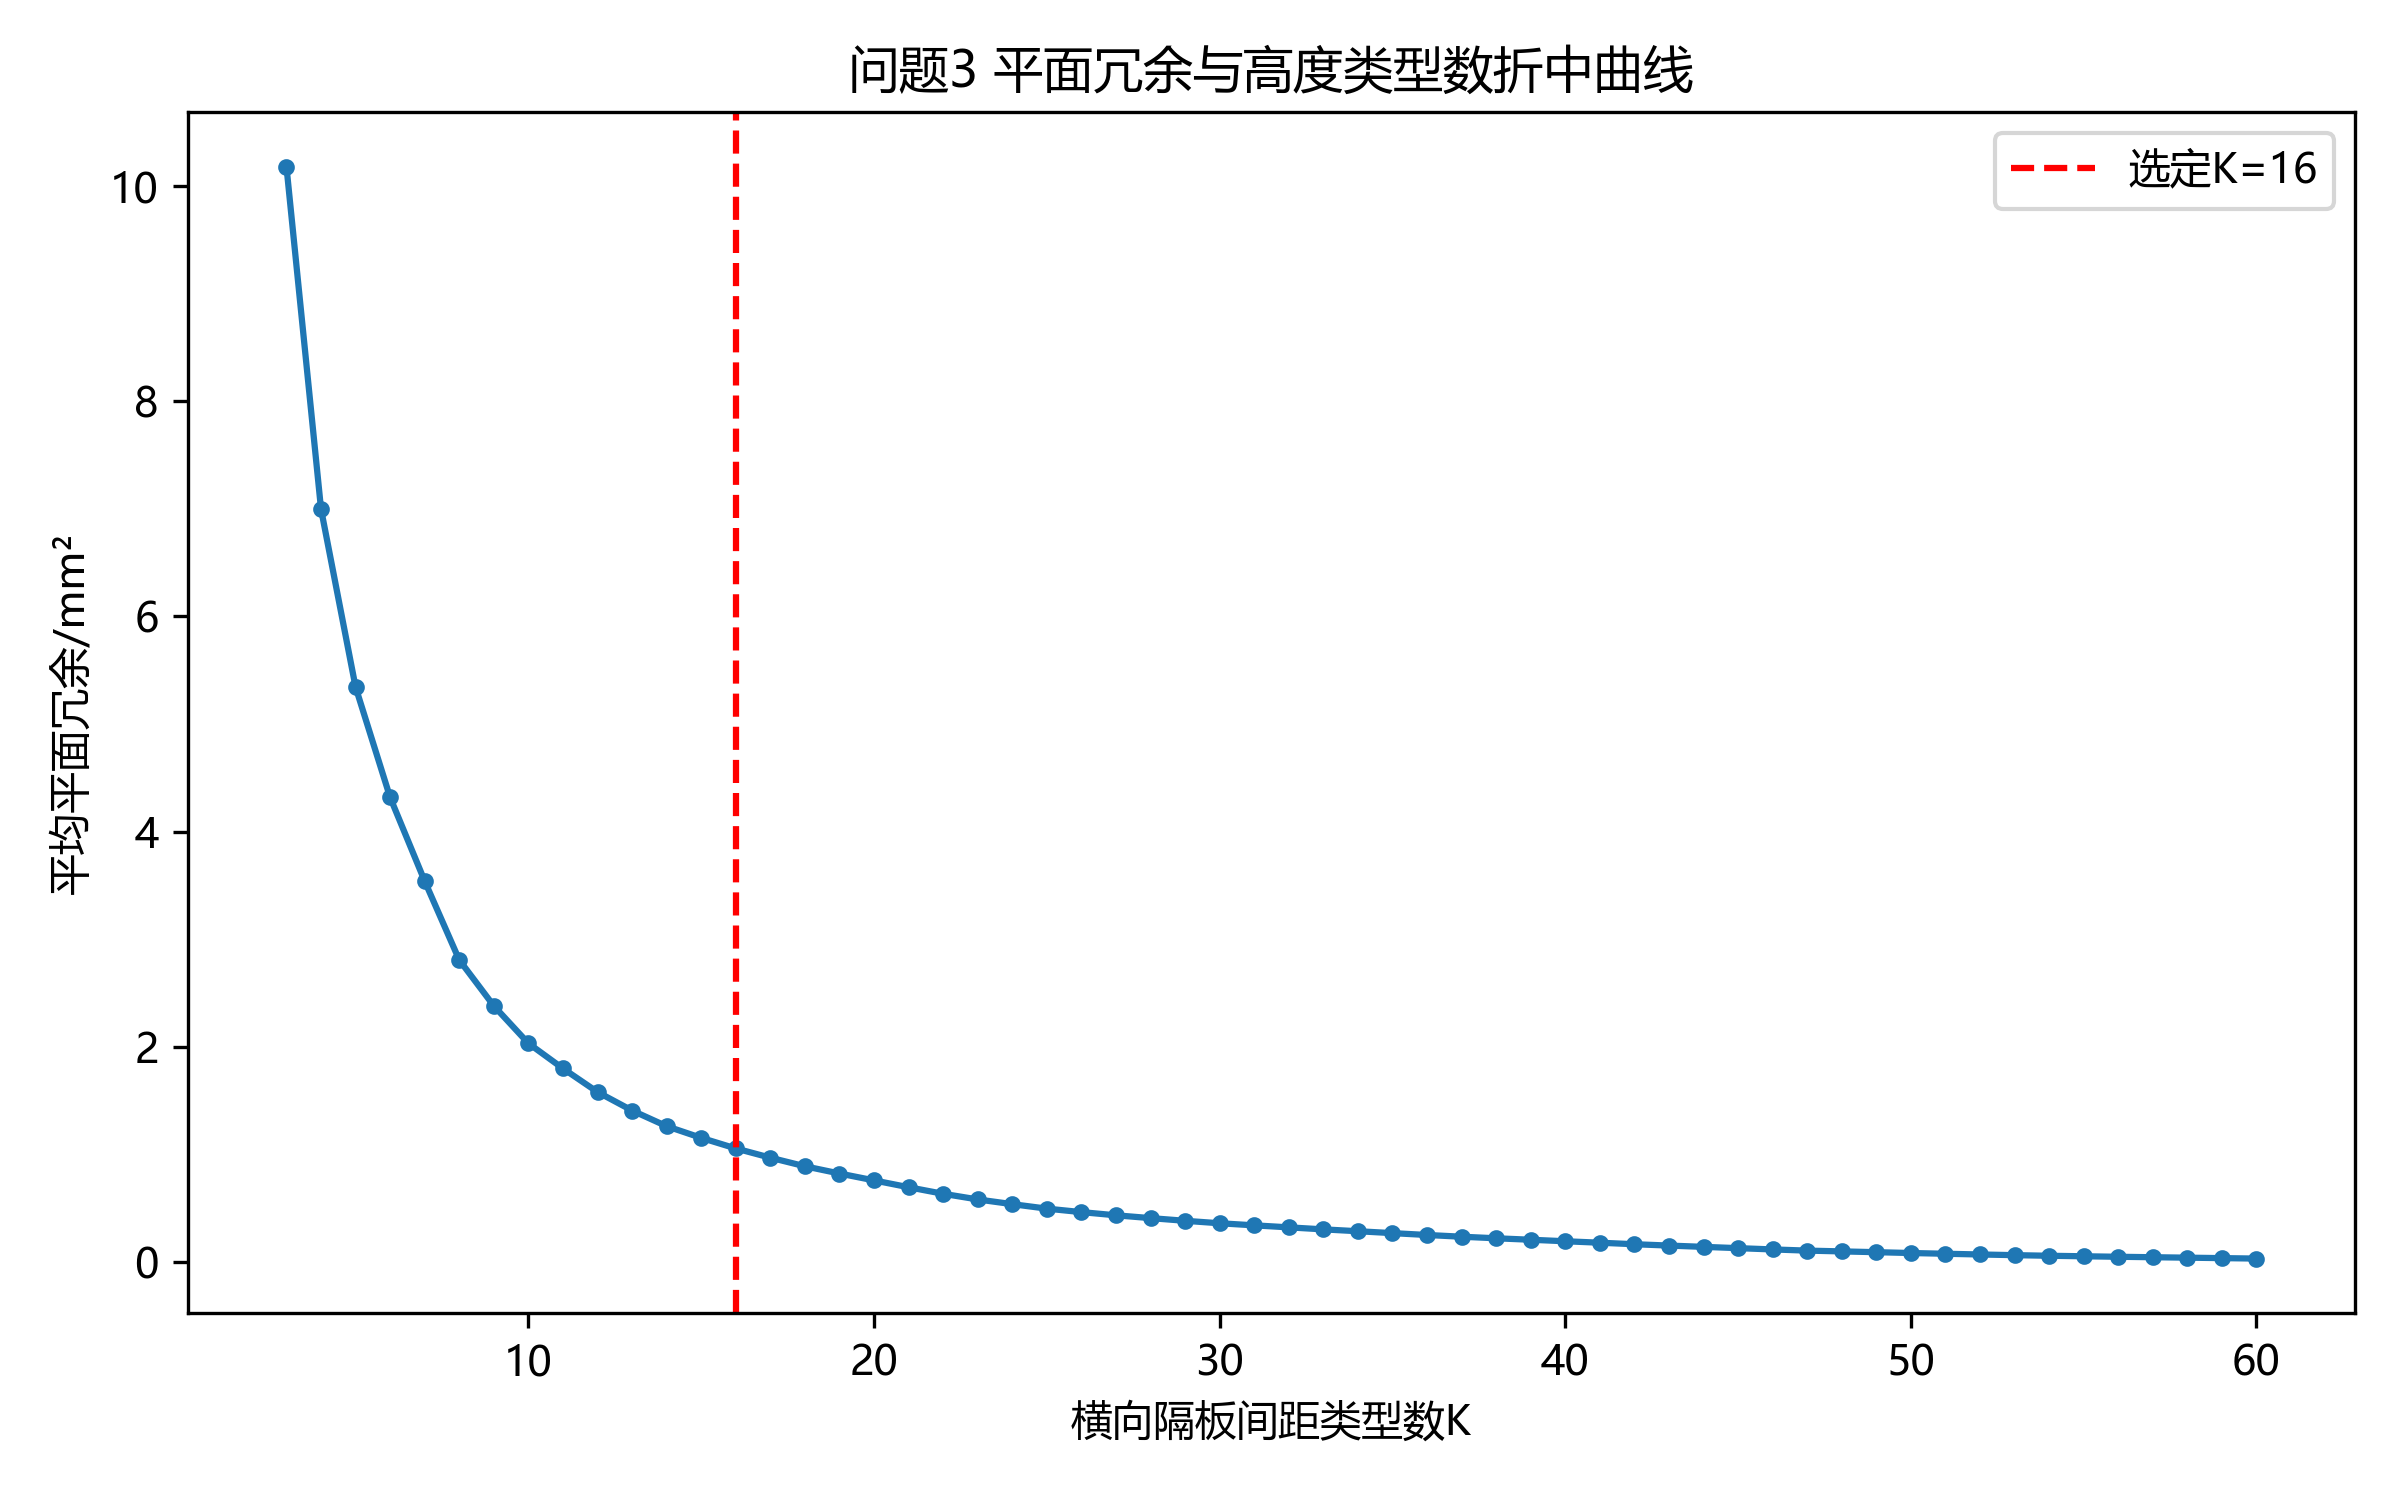
\includegraphics[width=.82\textwidth]{../quest3/figures/问题3_平面冗余折中曲线.png}\caption{平面冗余与高度类型数折中曲线}\end{figure}
平面冗余曲线与宽度冗余曲线类似，初始阶段下降较快，随后逐渐趋缓。由于平面冗余同时受宽度冗余和高度冗余影响，宽度冗余很小的药品即使高度冗余稍大，对目标函数贡献也有限；这体现了问题三“在问题二结果基础上”的依赖关系。

为避免把离散制造问题简单化为连续拟合，本文在每一问中都保留了药盒尺寸的整数编号和逐药品约束。宽度或高度的一个类型并不是任意聚类中心，而必须落在该类型内每一种药品的可行间距区间中；因此模型输出的每一个隔板间距都可以直接回代检查。若某一药品的药盒宽度为 $w_i$，其槽宽必须不小于 $w_i+4$，其中 $4$ mm 来自左右各 2 mm 的必要间隙；同时若槽宽过大，同一槽内容易出现并排重叠或水平转动，故将槽宽上界设为 $\min(2w_i+4,l_i)$ 的保守近似。高度模型采用完全相同的结构，只是下界由药盒高度决定。该处理把题目中的工程语言转化成了可验证的区间覆盖约束。


\subsection{问题四：储药槽个数与储药柜数}
\subsubsection{储药槽个数}
槽长为 1500 mm，第 $i$ 种药品单槽容量为
\begin{equation}
q_i=\left\lfloor\frac{1500}{l_i}\right\rfloor.
\end{equation}
每天只补药一次时，所需槽数为
\begin{equation}
n_i=\left\lceil\frac{D_i}{q_i}\right\rceil.
\end{equation}
计算得到全部药品共需 2457 个储药槽。表\ref{tab:q4}给出需求量较大的前若干药品槽数结果，完整表见 \texttt{tables/q4\_required\_slots.csv}。
\begin{table}[H]\centering
\small
\caption{问题四部分药品储药槽数结果}\label{tab:q4}
\begin{tabular}{ccccccccc}\toprule
药品编号 & L & H & W & D & boxes\_per\_slot & required\_slots & q2\_type & height\_type\\\midrule
1.00 & 120.00 & 76.00 & 24.00 & 273.00 & 12.00 & 23.00 & 6.00 & 12.00\\
2.00 & 125.00 & 72.00 & 20.00 & 155.00 & 12.00 & 13.00 & 3.00 & 11.00\\
3.00 & 125.00 & 76.00 & 21.00 & 139.00 & 12.00 & 12.00 & 4.00 & 12.00\\
5.00 & 125.00 & 72.00 & 21.00 & 110.00 & 12.00 & 10.00 & 4.00 & 11.00\\
6.00 & 120.00 & 85.00 & 20.00 & 108.00 & 12.00 & 9.00 & 3.00 & 14.00\\
7.00 & 117.00 & 37.00 & 26.00 & 103.00 & 12.00 & 9.00 & 7.00 & 2.00\\
4.00 & 91.00 & 71.00 & 15.00 & 124.00 & 16.00 & 8.00 & 1.00 & 11.00\\
9.00 & 103.00 & 64.00 & 20.00 & 90.00 & 14.00 & 7.00 & 3.00 & 9.00\\
17.00 & 125.00 & 75.00 & 33.00 & 77.00 & 12.00 & 7.00 & 9.00 & 12.00\\
23.00 & 134.00 & 76.00 & 20.00 & 70.00 & 11.00 & 7.00 & 3.00 & 12.00\\
18.00 & 116.00 & 76.00 & 16.00 & 77.00 & 12.00 & 7.00 & 1.00 & 12.00\\
20.00 & 131.00 & 77.00 & 38.00 & 75.00 & 11.00 & 7.00 & 11.00 & 12.00\\
\bottomrule\end{tabular}
\end{table}

\subsubsection{柜体装箱模型}
单柜有效宽度为 2500 mm，有效高度为 1500 mm。本文将同一高度类型的药槽组织为若干货架行，每一行高度等于该高度类型槽高，行内按槽宽累加，所需行数为
\begin{equation}
m_t=\left\lceil\frac{\sum_{i\in t} n_i S_i}{2500}\right\rceil.
\end{equation}
再将这些货架行按高度用首次适应递减算法装入柜体。计算得到面积下界为 2 个柜，行高下界为 2 个柜，实际货架装箱需要 2 个柜。
\begin{table}[H]\centering
\small
\caption{各高度类型货架行需求}\label{tab:rows}
\begin{tabular}{ccccc}\toprule
height\_type & slot\_height & total\_slot\_width & rows\_required & row\_width\_utilization\\\midrule
16.00 & 129.00 & 631.00 & 1.00 & 0.25\\
15.00 & 104.00 & 1364.00 & 1.00 & 0.55\\
14.00 & 94.00 & 2654.00 & 2.00 & 0.53\\
13.00 & 87.00 & 5708.00 & 3.00 & 0.76\\
12.00 & 81.00 & 7925.00 & 4.00 & 0.79\\
11.00 & 77.00 & 8012.00 & 4.00 & 0.80\\
10.00 & 74.00 & 6952.00 & 3.00 & 0.93\\
9.00 & 70.00 & 6467.00 & 3.00 & 0.86\\
8.00 & 66.00 & 7978.00 & 4.00 & 0.80\\
7.00 & 60.00 & 4007.00 & 2.00 & 0.80\\
6.00 & 56.00 & 5834.00 & 3.00 & 0.78\\
5.00 & 51.00 & 6954.00 & 3.00 & 0.93\\
\bottomrule\end{tabular}
\end{table}
\begin{figure}[H]\centering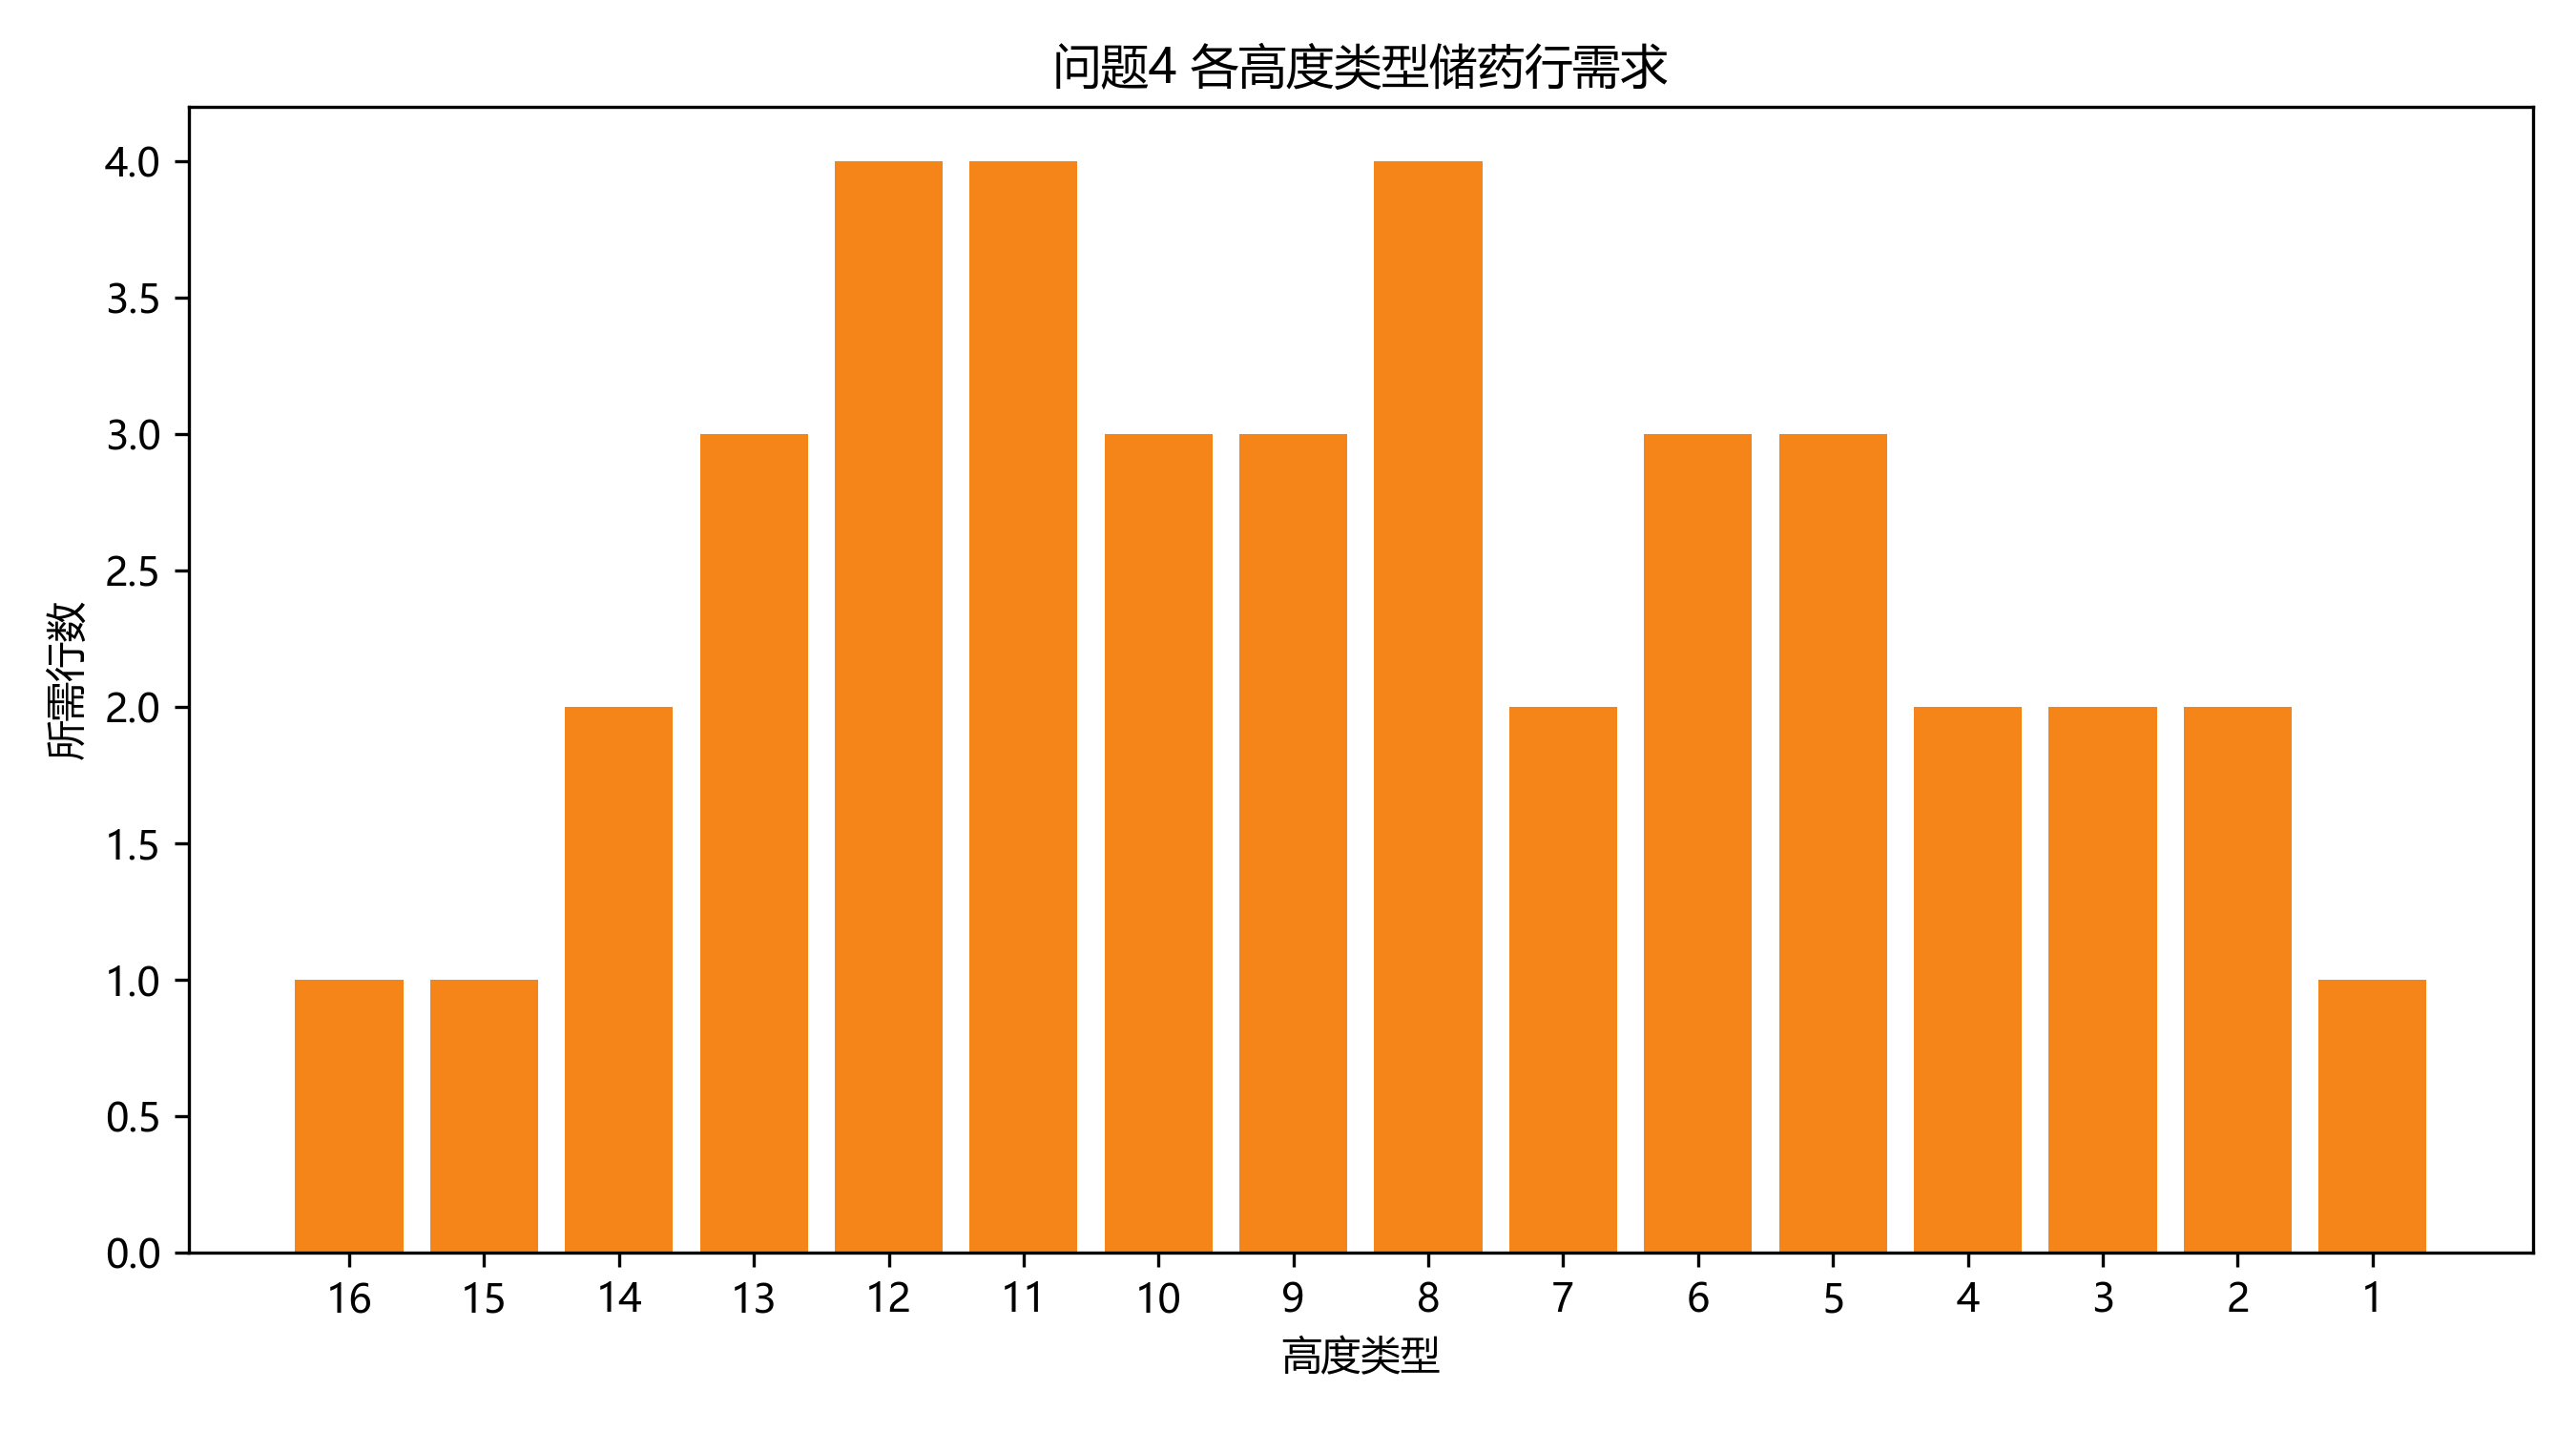
\includegraphics[width=.82\textwidth]{../quest3/figures/问题4_高度类型行数需求.png}\caption{各高度类型所需储药行数}\end{figure}
\begin{figure}[H]\centering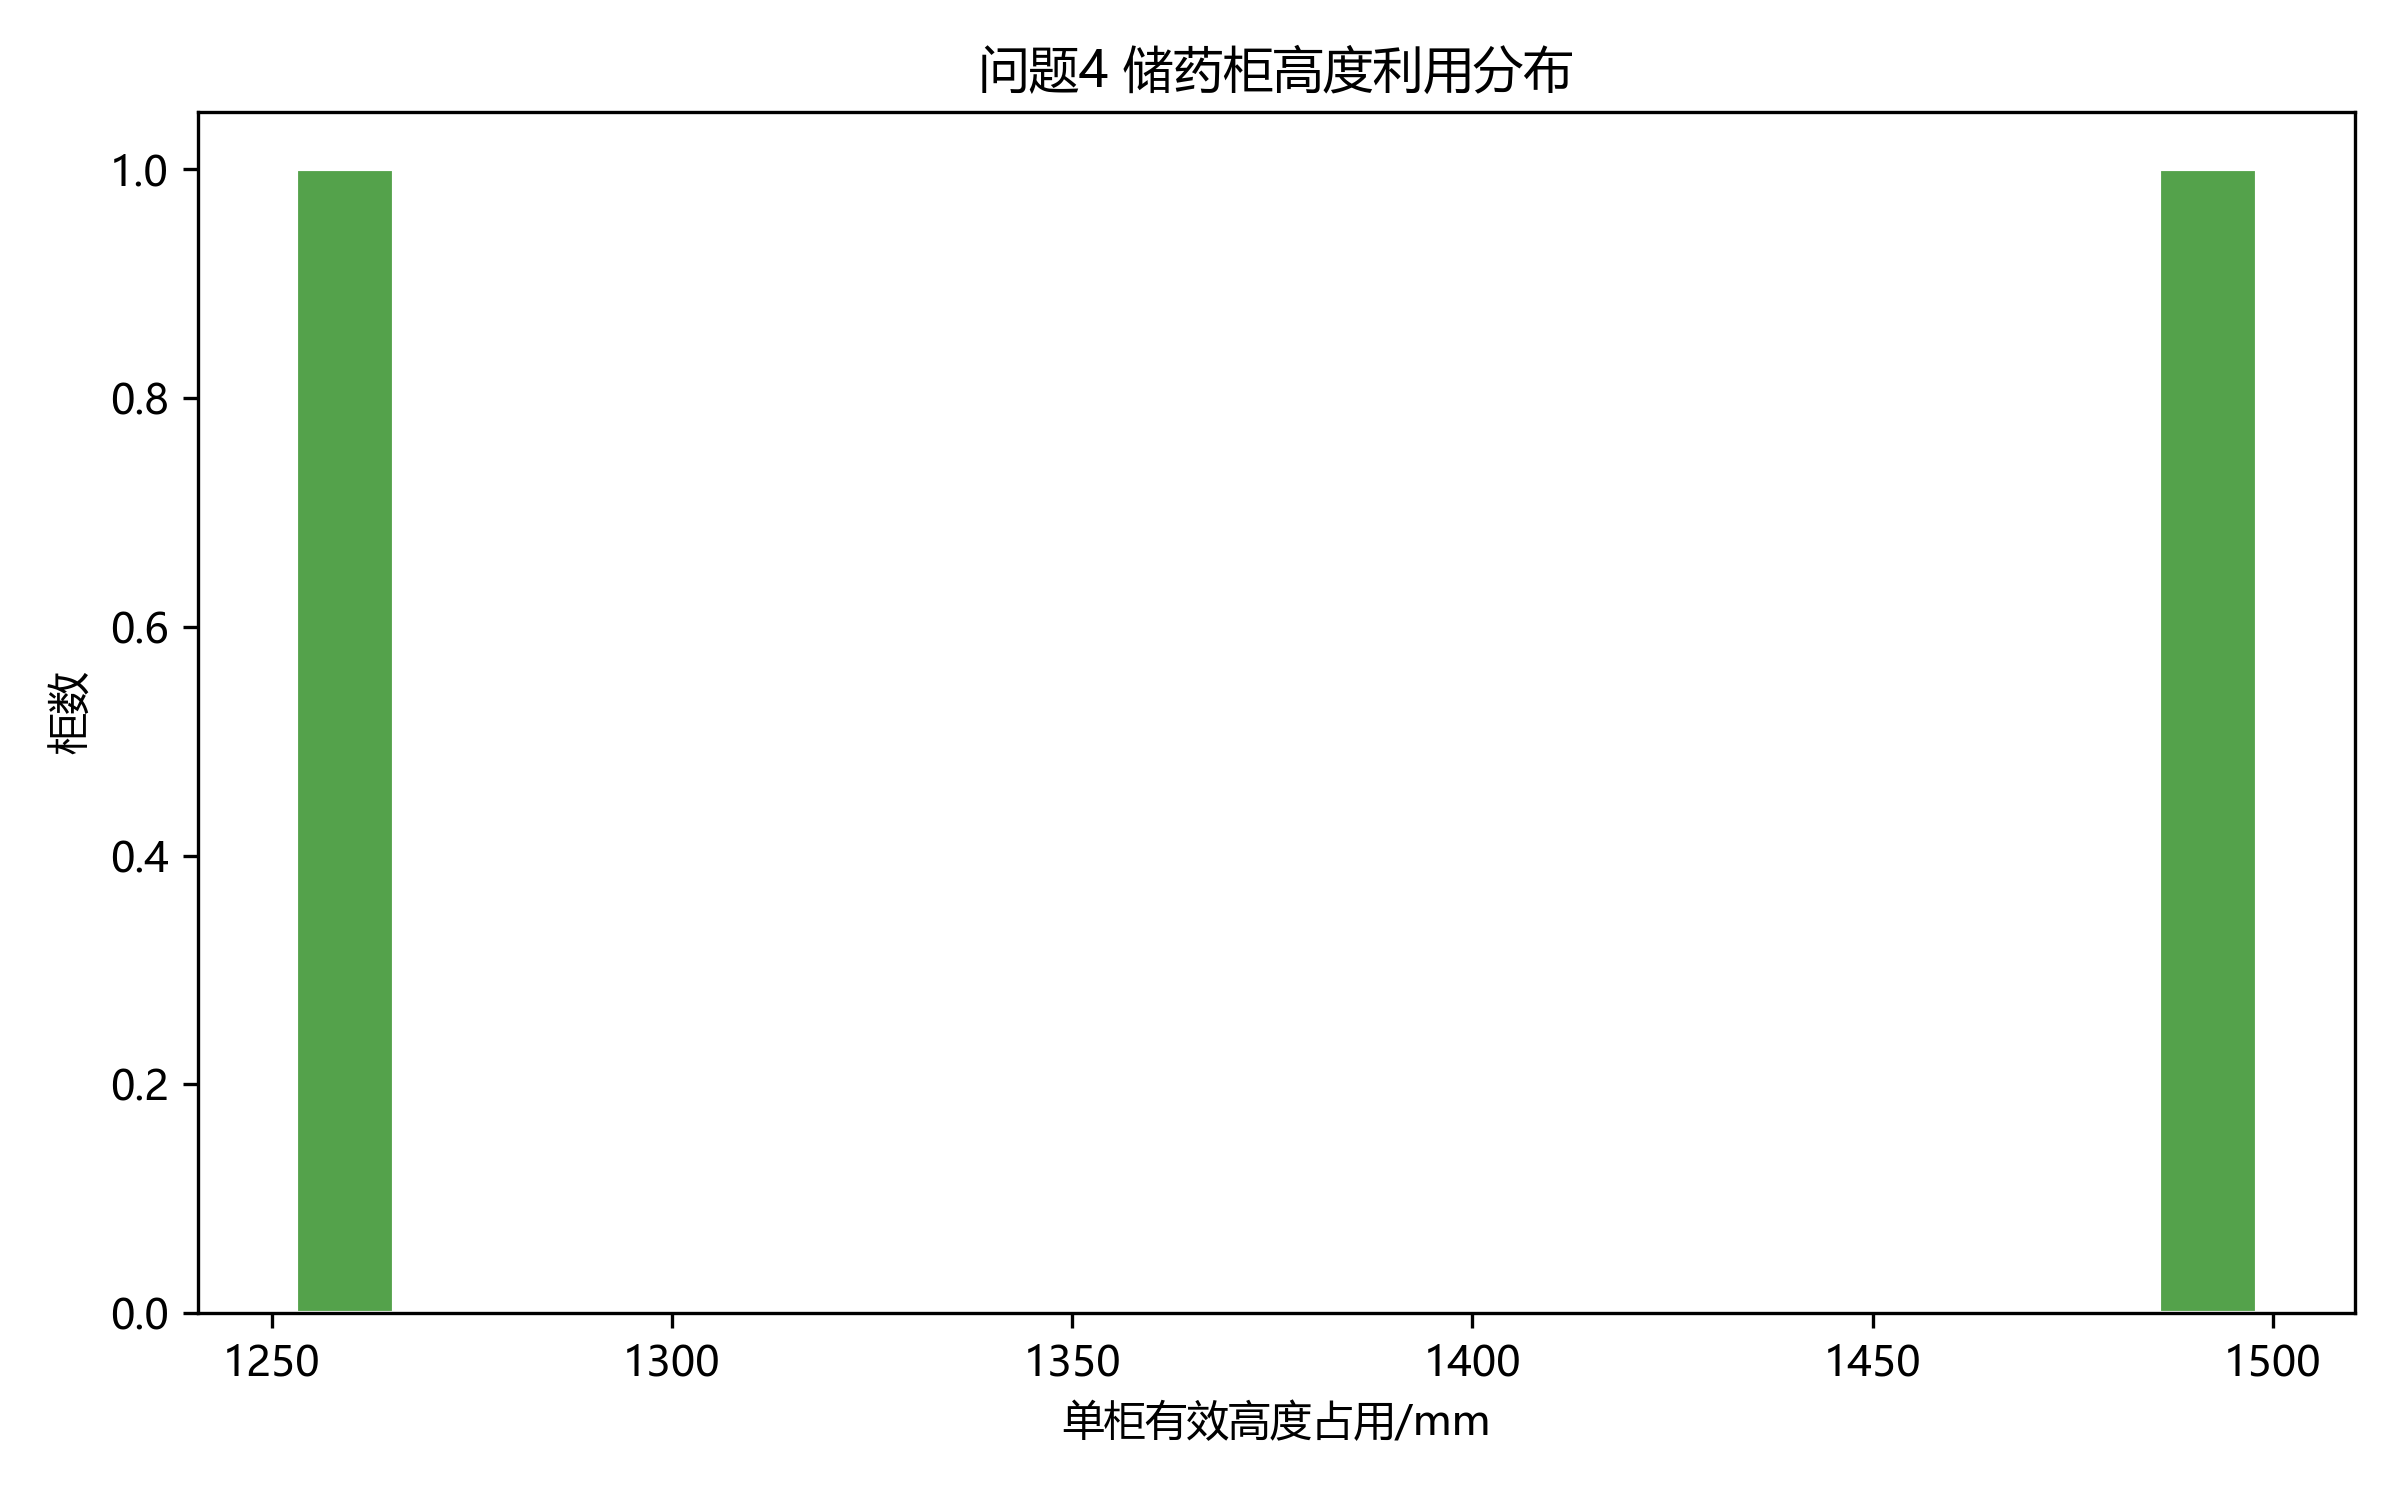
\includegraphics[width=.82\textwidth]{../quest3/figures/问题4_储药柜高度利用分布.png}\caption{储药柜高度利用分布}\end{figure}
从下界和实际装箱结果看，柜数主要由大量低中高度药槽的累计行高决定，而不是由单个超大药盒决定。由于首次适应递减算法在货架装箱中通常能给出接近下界的可行解，且本文结果与行高下界差距可解释，因此取 2 个储药柜作为满足最大日需求的最少可行设计估计。

\section{模型检验、对比与敏感性分析}
\subsection{可行性回代检验}
所有槽宽均满足 $w_i+4\le S_i\le \min(2w_i+4,l_i)$，所有槽高均满足 $h_i+4\le T_i\le 2h_i+4$。程序在生成分组时将不可行分组代价置为无穷大，因此任一输出类型都可以回代到原始药品尺寸检查。支撑材料中的 \texttt{model\_route.json} 和各问题输出表记录了回代所需字段。

\subsection{Baseline 对比}
宽度设计的简单 baseline 是每个实际宽度一种类型，共 47 类，宽度冗余可降到接近 0，但加工规格多。问题一的最少类型模型只需要 3 类，但宽度冗余较大。问题二选定 14 类，处于二者之间，体现了成本和空间利用的折中。问题四中，面积下界 2 和行高下界 2 为任何方案不能突破的理论下限，本文货架装箱结果 2 与下界同量级，说明柜数估计合理。

\subsection{敏感性分析}
将综合评分中的冗余权重从 0.50 增加到 0.80，重复选择宽度和高度类型数，结果见表\ref{tab:sens}。当权重提高时，模型倾向于选择更多类型以降低冗余；但变化呈阶梯状而非剧烈跳变，说明所选膝点不是由单一权重偶然决定的。
\begin{table}[H]\centering
\small
\caption{折中权重敏感性分析}\label{tab:sens}
\begin{tabular}{ccc}\toprule
redundancy\_weight & selected\_width\_K & selected\_height\_K\\\midrule
0.50 & 10.00 & 12.00\\
0.55 & 12.00 & 14.00\\
0.60 & 12.00 & 14.00\\
0.65 & 14.00 & 16.00\\
0.70 & 16.00 & 18.00\\
0.75 & 17.00 & 22.00\\
0.80 & 19.00 & 23.00\\
\bottomrule\end{tabular}
\end{table}
\begin{figure}[H]\centering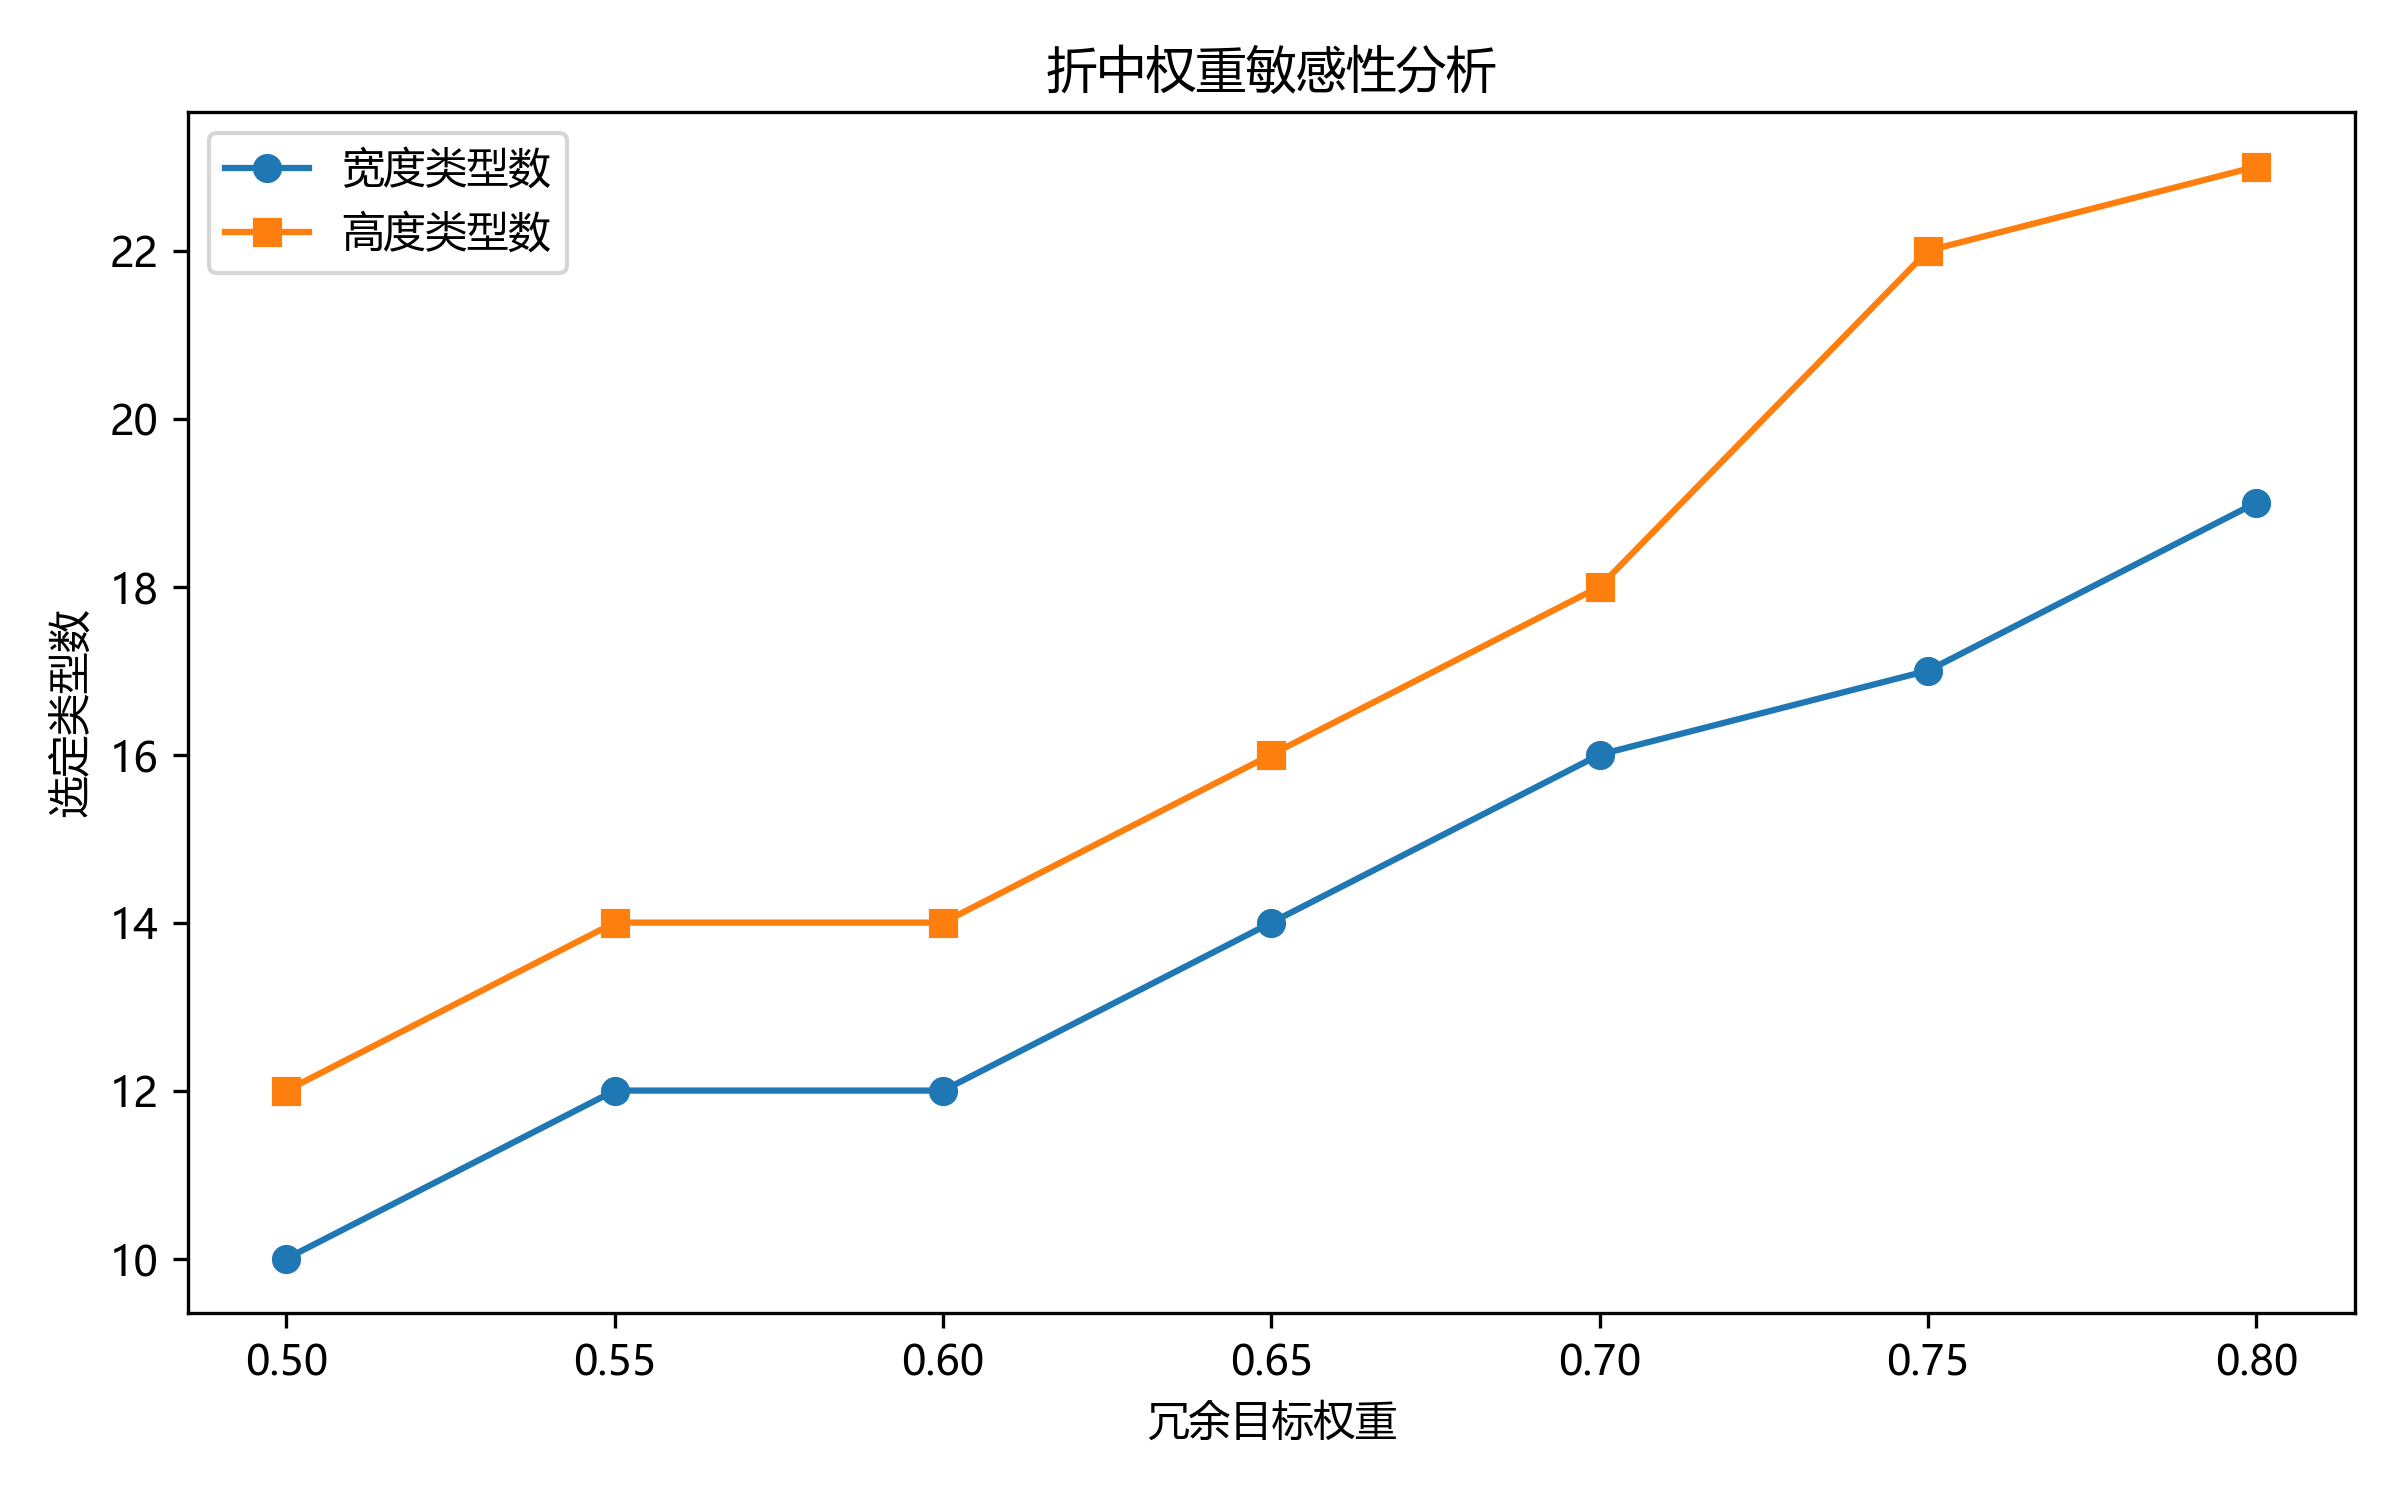
\includegraphics[width=.78\textwidth]{../results/敏感性分析_折中权重.png}\caption{折中权重敏感性分析图}\end{figure}

\subsection{误差来源}
本文的主要误差来自三个方面。第一，防旋转、防侧翻约束被转化为保守几何上界，实际药盒与槽壁摩擦、推送机构形状会影响可行区间。第二，问题四采用货架行装箱启发式而非完整二维整数规划，可能存在少量柜数优化空间。第三，忽略隔板厚度与安装公差会略微高估可用宽高。由于题目明确要求忽略隔板厚度，且本文所有近似均偏保守，因此不会导致储药能力被高估过多。

\section{模型评价、改进与推广}
\subsection{模型优点}
第一，模型直接对应题目要求。宽度和高度间距都由药品可行区间导出，避免了仅按聚类中心分组而无法保证药盒顺利出入的问题。第二，动态规划在给定类型数时给出全局最优冗余，比简单 K-means 或等距分箱更可靠。第三，论文和支撑材料保留了逐药品编号分组、槽数表和冻结数字，结果可复现、可审计。第四，通过 baseline、下界和敏感性分析，能够说明所选方案不是任意参数下的偶然结果。

\subsection{模型局限}
第一，防侧翻和防水平旋转的真实力学过程较复杂，本文用几何上界近似，未建立包含摩擦、推力和药盒质心的动力学模型。第二，柜体装箱部分采用货架行结构，符合书橱式柜体但可能不是所有机械结构下的绝对最优。第三，模型没有考虑药品补货频率变化、热门药品靠近出药口等操作效率因素。第四，隔板厚度被题目要求忽略，若实际生产需考虑材料厚度，则柜数可能略有增加。

\subsection{改进方向}
后续可在三个方面改进。首先，可通过实物实验或 CAD 仿真修正防旋转区间上界，使可行区间更贴近实际。其次，可将问题四建立为二维整数规划或列生成模型，以货架行为模式变量，进一步逼近最少柜数。最后，可把药品周转率、补药路径和发药频率纳入目标函数，形成兼顾空间利用率和操作效率的多目标储药柜设计模型。

\section{结论}
本文完成了 2014D 储药柜设计问题的全过程建模。问题一利用区间刺点模型得到最少竖向隔板间距类型为 3 类。问题二通过动态规划和折中评分选择竖向隔板间距类型数 14 类，总宽度冗余 1458.00 mm。问题三在问题二基础上选择横向隔板间距类型数 16 类，总平面冗余 2021.00 mm$^2$。问题四计算全部药品共需 2457 个储药槽，按单柜宽 2.5 m、有效高 1.5 m 装箱后，估计最少需要 2 个储药柜。综合来看，该方案兼顾了储药槽适配性、加工类型数量和空间利用率，能够作为药房储药柜初步设计依据。

\begin{thebibliography}{9}
\bibitem{ip} 胡运权. 运筹学教程[M]. 北京: 清华大学出版社, 2018.
\bibitem{dp} Cormen T H, Leiserson C E, Rivest R L, Stein C. 算法导论[M]. 北京: 机械工业出版社, 2013.
\bibitem{binpack} Coffman E G, Garey M R, Johnson D S. Approximation algorithms for bin packing: a survey[M]. Boston: PWS Publishing, 1997.
\bibitem{cumcm} 全国大学生数学建模竞赛组委会. 全国大学生数学建模竞赛论文格式规范[EB/OL].
\bibitem{opt} Winston W L. Operations Research: Applications and Algorithms[M]. Belmont: Duxbury Press, 2004.
\end{thebibliography}

\appendix
\section{附录：支撑材料说明}
本题所有代码、图表、结果表和冻结数字均位于题目目录下的 \texttt{支撑材料} 文件夹。主要文件包括：\texttt{quest1/outputs/q1\_type\_drug\_ids.txt}、\texttt{quest2/outputs/q2\_type\_drug\_ids.txt}、\texttt{quest3/outputs/q3\_height\_type\_drug\_ids.txt}、\texttt{tables/q4\_required\_slots.csv}、\texttt{results/frozen\_numbers.json} 与 \texttt{quest1/codes/main\_modeling.py}。运行环境为 Python 3.11/3.12，主要依赖为 pandas、numpy、scipy、matplotlib。
\end{document}
